
%%
%% forked from https://gits-15.sys.kt\mu \mu h.se/giampi/kthlatex kthlatex-0.2rc4 on 2020-02-13
%% expanded upon by Gerald Q. Maguire Jr.

%% Conventions for todo notes:
% \todo[inline]{Comments/directions/... in English}
% \todo[inline, backgroundcolor=kth-lightblue]{Text på svenska}
% \todo[inline, backgroundcolor=kth-lightgreen]{English descriptions about formatting}


% To optimize for digital output (this changes the color palette add the option: digitaloutput
\documentclass[english, biblatex, digitaloutput]{kththesis}

\usepackage[style=numeric,sorting=none,backend=biber]{biblatex}
%  \usepackage[bibstyle=authoryear, citestyle=authoryear,  maxbibnames=99, language=english]{biblatex}
\addbibresource{references.bib}


% include a variety of packages that are useful
%%%%%%%%%%%%%%%%%%%%%%%%%%%%%% Packages %%%%%%%%%%%%%%%%%%%%%%%%%%%%%%
%% The following are needed for generating the DiVA page(s)
\usepackage[force-eol=true]{scontents}              %% Needed to save lang, abstract, and keywords
\usepackage{pgffor}                 %% includes the foreach loop

%% Basic packages

%% Links
\usepackage{url}                %% Support for breaking URLs

%% Colorize
%\usepackage{color}
\PassOptionsToPackage{dvipsnames, svgnames}{xcolor}
\usepackage{xcolor}

\usepackage[normalem]{ulem}
\usepackage{soul}
\usepackage{xspace}
\usepackage{braket}

% to support units and decimal aligned columns in tables
% the option loads the binary prefixes
\usepackage[binary-units=true, locale=US]{siunitx}

\usepackage{balance}
\usepackage{stmaryrd}
\usepackage{booktabs}
\usepackage{graphicx}	        %% Support for images
\usepackage{multirow}	        %% Support for multirow columns in tables
\usepackage{tabularx}		    %% For simple table stretching
\usepackage{mathtools}
\usepackage{algorithm} 
\usepackage{algorithmic}  
\usepackage{amsmath}
\usepackage[linesnumbered,ruled,vlined,algo2e]{algorithm2e}
% can't use both algpseudocode and algorithmic packages
%\usepackage[noend]{algpseudocode}
%\usepackage{subfig}  %% cannot use both subcaption and subfig packages
\usepackage{optidef}
\usepackage{float}		        %% Support for more flexible floating box positioning
\usepackage{pifont}

%% some additional useful packages
% to enable rotated figures
\usepackage{rotating}	    	%% For text rotating
\usepackage{array}		        %% For table wrapping
\usepackage{mdwlist}            %% various list-related commands
\usepackage{setspace}           %% For fine-grained control over line spacing


\usepackage{enumitem}           %% to allow changes to the margins of descriptions


%% If you are going to include source code (or code snippets)
\usepackage{listings}		    %% For source code listing
%%\usepackage[cache=false]{minted} %% For source code highlighting
%%\usemintedstyle{borland}

\usepackage{bytefield}          %% For packet drawings


\setlength {\marginparwidth }{2cm} %leave some extra space for todo notes
\usepackage{todonotes}
\usepackage{notoccite} % do not number captions based on their appearance in the TOC


% Footnotes
\usepackage{perpage}
\usepackage[perpage,para,symbol]{footmisc} %% use symbols to ``number'' footnotes and reset which symbol is used first on each page


%% Various useful packages
%%----------------------------------------------------------------------------
%%   pcap2tex stuff
%%----------------------------------------------------------------------------
\usepackage{tikz}
\usetikzlibrary{arrows,decorations.pathmorphing,backgrounds,fit,positioning,calc,shapes}
\usepackage{pgfmath}	% --math engine
\newcommand\bmmax{2}
\usepackage{bm} % bold math


%% Managing titles
% \usepackage[outermarks]{titlesec}
%%%%%%%%%%%%%%%%%%%%%%%%%%%%%%%%%%%%%%%%%%%%%%%%%%%%%%%%%%%%%%%%%%%%%%
%\captionsetup[subfloat]{listofformat=parens}

% to include PDF pages
%\usepackage{pdfpages}


\usepackage{csquotes}               %% Recommended by biblatex
% to provide a float barrier use:
\usepackage{placeins}

\usepackage{comment}  %% Provides a comment environment
\usepackage{refcount}   %% to be able to get an expandable \getpagerefnumber


% for experiments with new cover
\usepackage{eso-pic}
\usepackage[absolute,overlay]{textpos}

\usepackage{xparse}  % to use for commands with optional arguments


%%% Local Variables:
%%% mode: latex
%%% TeX-master: t
%%% End:
% KTH colors for LaTeX documents
%
% Started from kthcolors by:
% Riccardo Sven Risuleo
% 2016-09-06 11:05:40
%
% from https://github.com/KTH-AC/kthcolors
%
% Adapted using the colors from "Graphic Profile Manual KTH" version 180604
% (i.e.. 2018-06-04) 
% see https://intra.kth.se/en/administration/kommunikation/grafiskprofil/kth-s-grafiska-profil-1.844676
% 
% G. Q. Maguire Jr.
% 2021-07-05
%

%\NeedsTexFormat{LaTeX2e}[1994/06/01]
%\ProvidesPackage{kthcolors}[2021/07/85 v3 Latex package with official KTH colors]

\RequirePackage{xcolor}
%% Primary colors
%% As of the new manual, there is only 1 primary color; but with three 
\definecolor{kth-blue}{RGB/cmyk}{25,84,166/0.849,0.494,0,0.349}
\colorlet{kth-blue80}{kth-blue!80!}
\colorlet{kth-blue40}{kth-blue!40!}

% these are no longer used as of 2018-06-04
%\definecolor{kth-red}{RGB/cmyk}{157,16,45/0,0.898,0.713,0.384}
%\definecolor{kth-green}{RGB/cmyk}{98,146,46/0.329,0,0.685,0.427}

%% Secondary colors
\definecolor{kth-lightblue}{RGB/cmyk}{36,160,216/0.833,0.259,0,0.153}
\colorlet{kth-lightblue80}{kth-lightblue!80!}
\colorlet{kth-lightblue40}{kth-lightblue!40!}

%\definecolor{kth-lightred}{RGB/cmyk}{228,54,62/0,0.763,0.728,0.106}
\definecolor{kth-lightred}{RGB}{216,84,151}
\colorlet{kth-lightred80}{kth-lightred!80!}
\colorlet{kth-lightred40}{kth-lightred!40!}

\definecolor{kth-lightgreen}{RGB/cmyk}{176,201,43/0.124,0,0.786,0.212} % olive
\colorlet{kth-lightgreen80}{kth-lightgreen!80!}
\colorlet{kth-lightgreen40}{kth-lightgreen!40!}

% Cool Gray 9C
%\definecolor{kth-coolgray}{RGB}{101,101,108}

% Cool Gray 10 suggested by Martin Krzywinski (see http://mkweb.bcgsc.ca/colorblind) 
\definecolor{kth-coolgray}{RGB}{99,102,106}
\colorlet{kth-coolgray80}{kth-coolgray!80!}
\colorlet{kth-coolgray40}{kth-coolgray!40!}

% Tertiary colors (yet more colors)
% All of these are no longer used
%\definecolor{kth-pink}{RGB/cmyk}{216,84,151/10,0.611,0.301,0.153}
%\definecolor{kth-yellow}{RGB/cmyk}{250,185,25/0,0.26,0.9,0.0196}
%\definecolor{kth-darkgray}{RGB/cmyk}{101,101,108/0.0648,0.0648,0,0.576}
%\definecolor{kth-middlegray}{RGB/cmyk}{189,188,188/0,0.00529,0.00529,0.259}
%\definecolor{kth-lightgray}{RGB/cmyk}{227,229,227/0.00873,0,0.00873,0.102}

%\DeclareOption{gray}{\colorlet{gray}{kth-darkgray}}

% These versions are designed to meet accessability requirements for digital media
% Note that the palette is more limited than for the print version of the colors
\ifdigitaloutput
    % primary color
    \definecolor{kth-blue}{HTML}{1954A6} % Deep sea
    \definecolor{kth-blue80}{HTML}{5E87C0}

    % Secondary colors
    \definecolor{kth-lightblue}{HTML}{2191C4} % Stratosphere
    \definecolor{kth-lightred}{HTML}{D02F80} % Fluorescence
    \definecolor{kth-lightred80}{HTML}{D95599}
    \definecolor{kth-lightgreen}{HTML}{62922E} % Front-lawn
    \definecolor{kth-coolgray}{HTML}{65656C} % Office
    \definecolor{kth-coolgray80}{HTML}{848489}
\fi


\makeatletter
\newcommand{\DeclareLatinAbbrev}[2]{%
  \DeclareRobustCommand{#1}{%
    \@ifnextchar{.}{\textit{#2}}{%
      \@ifnextchar{,}{\textit{#2.}}{%
        \@ifnextchar{!}{\textit{#2.}}{%
          \@ifnextchar{?}{\textit{#2.}}{%
            \@ifnextchar{)}{\textit{#2.}}{%
              {\textit{#2.,\ }}}}}}}}%
}
\makeatother
\DeclareLatinAbbrev{\eg}{e.g}
\DeclareLatinAbbrev{\Eg}{E.g}
\DeclareLatinAbbrev{\ie}{i.e}
\DeclareLatinAbbrev{\Ie}{I.e}
\DeclareLatinAbbrev{\etc}{etc}
\DeclareLatinAbbrev{\etal}{et~al}

\def\first {$(i)$\xspace}
\def\second{$(ii)$\xspace}
\def\third {$(iii)$\xspace}
\def\fourth{$(iv)$\xspace}
\def\fifth {$(v)$\xspace}
\def\sixth {$(vi)$\xspace}
\def\seventh{$(vii)$\xspace}
\def\eighth{$(viii)$\xspace}

%%% custom definitions
%% Coloring the links!
\newcommand\myshade{75} % Usage: red!\myshade!black

\definecolor{ForestGreen} {RGB}{34,  139,  34}
\definecolor{HeraldRed2}   {rgb}{0.81, 0.12, 0.15}

\newcommand{\refscolor} {blue}
\newcommand{\linkscolor}{HeraldRed2}
\newcommand{\urlscolor} {ForestGreen}

%% Some definitions of used colors
%\definecolor{darkblue}{rgb}{0.0,0.0,0.3} %% define a color called darkblue
%\definecolor{darkred}{rgb}{0.4,0.0,0.0}
%\definecolor{red}{rgb}{0.7,0.0,0.0}
%\definecolor{lightgrey}{rgb}{0.8,0.8,0.8} 
%\definecolor{grey}{rgb}{0.6,0.6,0.6}
%\definecolor{darkgrey}{rgb}{0.4,0.4,0.4}
%\definecolor{aqua}{rgb}{0.0, 1.0, 1.0}

% For runin headings
\newcommand{\smartparagraph}[1]{\vspace{.05in}\noindent\textbf{#1}}

%% Table of Contents (ToC) depth 
\setcounter{secnumdepth}{4} % how many sectioning levels to assign numbers to
\setcounter{tocdepth}{4}    % how many sectioning levels to show in ToC

%% Limit hyphenation
\hyphenpenalty=9000
\tolerance=5000
% Reduce hyphenation as much as possible:
%\hyphenpenalty=15000
%\tolerance=1000

% For notes by the authors to themselves
\newcommand*{\todoinline}[1]{\textcolor{red}{TODO: #1}}
  % load some additional definitions to make writing more consistent

% The following is needed in conjunction with generating the DiVA data with abstracts and keywords using the scontents package and a modified listings environment
%\usepackage{listings}   %  already included
\ExplSyntaxOn
\newcommand\typestoredx[2]{\expandafter\__scontents_typestored_internal:nn\expandafter{#1} {#2}}
\ExplSyntaxOff
\makeatletter
\let\verbatimsc\@undefined
\let\endverbatimsc\@undefined
\lst@AddToHook{Init}{\hyphenpenalty=50\relax}
\makeatother


\lstnewenvironment{verbatimsc}
    {
    \lstset{%
        basicstyle=\ttfamily\tiny,
        backgroundcolor=\color{white},
        %basicstyle=\tiny,
        %columns=fullflexible,
        columns=[l]fixed,
        language=[LaTeX]TeX,
        %numbers=left,
        %numberstyle=\tiny\color{gray},
        keywordstyle=\color{red},
        breaklines=true,                 % sets automatic line breaking
        breakatwhitespace=true,          % sets if automatic breaks should only happen at whitespace
        %keepspaces=false,
        breakindent=0em,
        %fancyvrb=true,
        frame=none,                     % turn off any box
        postbreak={}                    % turn off any hook arrow for continuation lines
    }
}{}



%% definition of new command for bytefield package
\newcommand{\colorbitbox}[3]{%
	\rlap{\bitbox{#2}{\color{#1}\rule{\width}{\height}}}%
	\bitbox{#2}{#3}}

%% Acronyms
% note that nonumberlist - removes the cross references to the pages where the acronym appears
% note that nomain - does not produce a main glossary, this only acronyms will be in the glossary
% note that nopostdot - will present there being a period at the end of each entry
\usepackage[acronym, section=section, nonumberlist, nomain, nopostdot]{glossaries}
\usepackage[automake]{glossaries-extra}
\setabbreviationstyle[acronym]{long-short}  % for use with the glossaries.extra package, causes the acronym to be spelled out on first use

\usepackage[plainpages=false]{hyperref}  % Because backref is not compatible with biblatex
\usepackage[all]{hypcap}  % prevents an issue related to hyperref and caption linking


% packages that have to be included after hyperref
\usepackage{doi}
\usepackage{cleveref}           %% Replace Section with a symbol


%\glsdisablehyper
\makeglossaries
%%% Local Variables:
%%% mode: latex
%%% TeX-master: t
%%% End:

% % The form of the entries in this file is \newacronym{label}{acronym}{phrase}
% %                                      or \newacronym[options]{label}{acronym}{phrase}
% % see "User Manual for glossaries.sty" for the  details about the options, one example is shown below
% % note the specification of the long form plural in the line below
% \newacronym[longplural={Debugging Information Entities}]{DIE}{DIE}{Debugging Information Entity}
% %
% % The following example also uses options
% \newacronym[plural={OSes}, firstplural={operating systems (OSes)}]{OS}{OS}{operating system}

% % note the use of a non-breaking dash in long text for the following acronym
% \newacronym{IQL}{IQL}{Independent Q‑Learning}

% \newacronym{LAN}{LAN}{Local Area Network}
% % note the use of a non-breaking dash in the following acronym
% \newacronym{WiFi}{Wi-Fi}{Wireless Fidelity}

% \newacronym{WLAN}{WLAN}{Wireless Local Area Network}
% \newacronym{UN}{UN}{United Nations}
% \newacronym{SDG}{SDG}{Sustainable Development Goal}

%%%%%%%%%% Start %%%%%%%%%

\newacronym[longplural={Distributed Ledger Technologies}]{DLT}{DLT}{Distributed Ledger Technology}
\newacronym{RDBMS}{RDBMS}{Relational Database Management System}
\newacronym{P2P}{P2P}{Peer-to-peer}
\newacronym{PGP}{PGP}{Pretty Good Privacy}
\newacronym{PKI}{PKI}{Public Key Infrastructure}
\newacronym{CIA}{CIA}{Confidentiality, Integrity, Availability}
\newacronym{FOSS}{FOSS}{Free Open Source Software}
\newacronym{MSP}{MSP}{Membership Service Provider}
\newacronym[longplural={Certificate Authorities}]{CA}{CA}{Certificate Authority}  %load the acronyms file

%% Information for inside title page
\title{Trust in your friends, on the ledger}
\subtitle{Safer reproducible builds through decentralized distribution of .buildinfo files}

% give the alternative title - i.e., if the thesis is in English, then give a Swedish title
\alttitle{Detta är den svenska översättningen av titeln}
\altsubtitle{Detta är den svenska översättningen av undertiteln}

\authorsLastname{Moritz}
\authorsFirstname{Johan}
\email{jmoritz@kth.se}
\kthid{u100001}
% As per email from KTH Biblioteket on 2021-06-28 students cannot have an OrCiD reported for their degree project
\authorsSchool{\schoolAcronym{EECS}}

% If there is a second author - add them here:
% \secondAuthorsLastname{Student}
% \secondAuthorsFirstname{Fake B.}
% \secondemail{b@kth.se}
% \secondkthid{u100002}
% % As per email from KTH Biblioteket on 2021-06-28 students cannot have an OrCiD reported for their degree project
% \secondAuthorsSchool{\schoolAcronym{ABE}}

\supervisorAsLastname{Nebbione}
\supervisorAsFirstname{Giuseppe}
\supervisorAsEmail{nebbione@kth.se}
% If the supervisor is from within KTH add their KTHID, School and Department info
\supervisorAsKTHID{u100003}
\supervisorAsSchool{\schoolAcronym{EECS}}
\supervisorAsDepartment{Computer Science}
% other for a supervisor outside of KTH add their organization info
%\supervisorAsOrganization{Timbuktu University, Department of Pseudoscience}

% %If there is a second supervisor add them here:
% \supervisorBsLastname{Supervisor}
% \supervisorBsFirstname{Another Busy}
% \supervisorBsEmail{sb@kth.se}
% % If the supervisor is from within KTH add their KTHID, School and Department info
% \supervisorBsKTHID{u100003}
% \supervisorBsSchool{\schoolAcronym{ABE}}
% \supervisorBsDepartment{Architecture}
% % other for a supervisor outside of KTH add their organization info
% %\supervisorBsOrganization{Timbuktu University, Department of Pseudoscience}

% %If there is a third supervisor add them here:
% \supervisorCsLastname{Supervisor}
% \supervisorCsFirstname{Third Busy}
% \supervisorCsEmail{sc@tu.va}
% % If the supervisor is from within KTH add their KTHID, School and Department info
% %\supervisorCsKTHID{u100004}
% %\supervisorCsSchool{\schoolAcronym{ABE}}
% %\supervisorCsDepartment{Public Buildings}
% % other for a supervisor outside of KTH add their organization info
% \supervisorCsOrganization{Timbuktu University, Department of Pseudoscience}

\examinersLastname{Dam}
\examinersFirstname{Mads}
\examinersEmail{mfd@kth.se}
% If the examiner is from within KTH add their KTHID, School and Department info
\examinersKTHID{u1d13i2c}
\examinersSchool{\schoolAcronym{EECS}}
\examinersDepartment{Computer Science}
% other for a examiner outside of KTH add their organization info
%\examinersOrganization{Timbuktu University, Department of Pseudoscience}


\hostcompany{Företaget AB} % Remove this line if the project was not done at a host company
%\hostorganization{CERN}   % if there was a host organization


\date{\today}

% For a CDATE student the following are likely values:
\programcode{CDATE}
\courseCycle{2}
\courseCode{DA231X}
\courseCredits{30.0}
\degreeName{Degree of Master of Science in Engineering}
\subjectArea{Computer Science and Engineering}

%%%%% For the oral presentation
%% Add this information once your examiner has scheduled your oral presentation
\presentationDateAndTimeISO{2021-03-15 13:00}
\presentationLanguage{eng}
\presentationRoom{via Zoom https://kth-se.zoom.us/j/ddddddddddd}
\presentationAddress{Isafjordsgatan 22 (Kistagången 16)}
\presentationCity{Stockholm}

% When there are multiple opponents, separate their names with '\&'
% Opponent's information
\opponentsNames{A. B. Normal \& A. X. E. Normalè}

%%%%% for DiVA's National Subject Category information
%%% Enter one or more 3 or 5 digit codes
%%% See https://www.scb.se/contentassets/3a12f556522d4bdc887c4838a37c7ec7/standard-for-svensk-indelning--av-forskningsamnen-2011-uppdaterad-aug-2016.pdf
%%% See https://www.scb.se/contentassets/10054f2ef27c437884e8cde0d38b9cc4/oversattningsnyckel-forskningsamnen.pdf
%%%%
%%%% Some examples of these codes are shown below:
% 102 Data- och informationsvetenskap (Datateknik)    Computer and Information Sciences
% 10201 Datavetenskap (datalogi) Computer Sciences 
% 10202 Systemvetenskap, informationssystem och informatik (samhällsvetenskaplig inriktning under 50804)
% Information Systems (Social aspects to be 50804)
% 10203 Bioinformatik (beräkningsbiologi) (tillämpningar under 10610)
% Bioinformatics (Computational Biology) (applications to be 10610)
% 10204 Människa-datorinteraktion (interaktionsdesign) (Samhällsvetenskapliga aspekter under 50803) Human Computer Interaction (Social aspects to be 50803)
% 10205 Programvaruteknik Software Engineering
% 10206 Datorteknik Computer Engineering
% 10207 Datorseende och robotik (autonoma system) Computer Vision and Robotics (Autonomous Systems)
% 10208 Språkteknologi (språkvetenskaplig databehandling) Language Technology (Computational Linguistics)
% 10209 Medieteknik Media and Communication Technology
% 10299 Annan data- och informationsvetenskap Other Computer and Information Science
%%%
% 202 Elektroteknik och elektronik Electrical Engineering, Electronic Engineering, Information Engineering
% 20201 Robotteknik och automation Robotics
% 20202 Reglerteknik Control Engineering
% 20203 Kommunikationssystem Communication Systems
% 20204 Telekommunikation Telecommunications
% 20205 Signalbehandling Signal Processing
% 20206 Datorsystem Computer Systems
% 20207 Inbäddad systemteknik Embedded Systems
% 20299 Annan elektroteknik och elektronik Other Electrical Engineering, Electronic Engineering, Information Engineering
%% Example for a thesis in Computer Science and Computer Systems
\nationalsubjectcategories{10201, 10206}

% for entering the TRITA number for a thesis
\trita{TRITA-EECS-EX}{2021:00}

% Enter the English and Swedish keywords here for use in the PDF meta data _and_ for later use
% following the respective abstract.
% Try to put the words in the same order in both languages to facilitate matching. For example:
\EnglishKeywords{Keyword 1, Keyword 2, Keyword3}
\SwedishKeywords{Nyckelord 1, Nyckelord 2, Nyckelord 3}

% Put the title, author, and keyword information into the PDF meta information
% This file contains the LaTeX to add information to the PDF file (specifically, author(s), title(s), and keywords
% It uses the hyperref package and should be be included before the \begin{document}
%
% I want to acknowledge the inspiration of Karl Voit's template for TU Graz that inspired me to add the PDF document information
% For more information about his template see https://github.com/novoid/LaTeX-KOMA-template
% Note that this template does not use anything from his template other than the names of the information for the PDF meta fields, i.e., mytitle, myauthor, and mykeywords together with the idea of defining the corresponding newcommand to set the relevant hyperref parameters.

\makeatletter
\ifx\@subtitle\@empty
    \newcommand{\mytitle}{\@title}
\else
    \newcommand{\mytitle}{\@title: \@subtitle}
\fi
\makeatother

\hypersetup{
     pdftitle={\mytitle}        % Title field
}

\makeatletter
\ifx\@secondAuthorsLastname\@empty
    \newcommand{\myauthor}{\@authorsFirstname\space\@authorsLastname} 
\else
    \ifinswedish
    \newcommand{\myauthor}{\@authorsFirstname\space\@authorsLastname\space\relax och\space\@secondAuthorsFirstname \@secondAuthorsLastname}
    \else
        \newcommand{\myauthor}{\@authorsFirstname\space\@authorsLastname\space\relax and\space\@secondAuthorsFirstname \@secondAuthorsLastname}
    \fi
\fi
\makeatother

\hypersetup{
     pdfauthor={\myauthor}      % Author field
}

% Put the alternative title (and subtitle) into the PDF Subject meta
\makeatletter
\ifx\@altsubtitle\@empty\relax
    \newcommand{\myalttitle}{\@alttitle}
\else
    \newcommand{\myalttitle}{\@alttitle: \@altsubtitle}
\fi
\makeatother

\hypersetup{
     pdfsubject={\myalttitle}        % Subject field
}

\makeatletter
\ifx\@EnglishKeywords\@empty
    \ifx\@SwedishKeywords\@empty
        \newcommand{\mykeywords}{}
    \else
    \newcommand{\mykeywords}{\@SwedishKeywords}
    \fi
\else
    \ifx\@SwedishKeywords\@empty
        \newcommand{\mykeywords}{\@EnglishKeywords}
    \else
        \ifinswedish
            \newcommand{\mykeywords}{\@SwedishKeywords, \@EnglishKeywords}
        \else
            \newcommand{\mykeywords}{\@EnglishKeywords, \@SwedishKeywords}
        \fi
    \fi
\fi
\makeatother

\hypersetup{
     pdfkeywords={\mykeywords}        % Keywords field
}        
% I have _not_ set the following fields:
%    pdfcreator             % Creator field
%    pdfproducer            % Producer field
 


% the custom colors and the commands are defined in defines.tex    
\hypersetup{
	colorlinks  = true,
	breaklinks  = true,
	linkcolor   = \linkscolor,
	urlcolor    = \urlscolor,
	citecolor   = \refscolor,
	anchorcolor = black
}


\begin{document}
\selectlanguage{english}

%%% Set the numbering for the title page to a numbering series not in the preface or body
\pagenumbering{alph}
\kthcover
\titlepage
% document/book information page
\bookinfopage

% Frontmatter includes the abstracts and table-of-contents
\frontmatter
\setcounter{page}{1}
\begin{abstract}
	% The first abstract should be in the language of the thesis.
	% Abstract fungerar på svenska också.
	\markboth{\abstractname}{}
	\begin{scontents}[store-env=lang]
		eng
	\end{scontents}
	%%% The contents of the abstract (between the begin and end of scontents) will be saved in LaTeX format
	%%% and output on the page(s) at the end of the thesis with information for DiVA facilitating the correct
	%%% entry of the meta data for your thesis.
	%%% These page(s) will be removed before the thesis is inserted into DiVA.
	% One can save the abstract in a file by adding ", write-env=abstract-eng.tex"
	\begin{scontents}[store-env=abstracts,print-env=true]
		\todo[inline, backgroundcolor=kth-lightgreen]{All theses at KTH are \textbf{required} to have an abstract in both \textit{English} and \textit{Swedish}.}

		\todo[inline, backgroundcolor=kth-lightgreen]{Exchange students many want to include one or more abstracts in the language(s) used in their home institutions to avoid the need to write another thesis when returning to their home institution.}

		\todo[inline]{Keep in mind that most of your potential readers are only going to read your \texttt{title} and \texttt{abstract}. This is why it is important that the abstract give them enough information that they can decide is this document relevant to them or not. Otherwise the likely default choice is to ignore the rest of your document.\\

			A abstract should stand on its own, i.e., no citations, cross references to the body of the document, acronyms must be spelled out, \ldots .\\

			Write this early and revise as necessary. This will help keep you focused on what you are trying to do.}

		Write an abstract that is about 250 and 350 words (1/2 A4-page)  with the following components:: % key parts of the abstract
		\begin{itemize}
			\item What is the topic area? (optional) Introduces the subject area for the project.
			\item Short problem statement
			\item Why was this problem worth a Bachelor's/Master’s thesis project? (\ie, why is the problem both significant and of a suitable degree of difficulty for a Bachelor's/Master’s thesis project? Why has no one else solved it yet?)
			\item How did you solve the problem? What was your method/insight?
			\item Results/Conclusions/Consequences/Impact: What are your key results/\linebreak[4]conclusions? What will others do based upon your results? What can be done now that you have finished - that could not be done before your thesis project was completed?
		\end{itemize}
	\end{scontents}
	\clearpage
	\todo[inline, backgroundcolor=kth-lightgreen]{The following are some notes about what can be included (in terms of LaTeX) in your abstract. Note that since this material is outside of the scontents environment, it is not saved as part of the abstract; hence, it does not end up on the metadata at the end of the thesis.}
	Choice of typeface with \textbackslash textit, \textbackslash textbf, and \textbackslash texttt:  \textit{x}, \textbf{x}, and \texttt{x}

	Text superscripts and subscripts with \textbackslash textsubscript and \textbackslash textsuperscript: A\textsubscript{x} and A\textsuperscript{x}

	Some useful symbols: \textbackslash textregistered, \textbackslash texttrademark, and \textbackslash textcopyright. For example, copyright symbol: \textbackslash textcopyright Maguire 2021, and some superscripts: \textbackslash textsuperscript\{99m\}Tc, A\textbackslash textsuperscript\{*\}, A\textbackslash textsuperscript\{\textbackslash textregistered\}, and A\textbackslash texttrademark : \textcopyright Maguire 2021, and some superscripts: \textsuperscript{99m}Tc, A\textsuperscript{*}, A\textsuperscript{\textregistered}, and A\texttrademark. Another example: H\textbackslash textsubscript\{2\}O: H\textsubscript{2}O

	Simple environment with begin and end: itemize and enumerate and within these \textbackslash item

	The following macros can be used: \textbackslash eg, \textbackslash Eg, \textbackslash ie, \textbackslash Ie, \textbackslash etc, and \textbackslash etal: \eg, \Eg, \ie, \Ie, \etc, and \etal

	The following macros for numbering with lower case roman numerals: \textbackslash first, \textbackslash second, \textbackslash third, \textbackslash fourth, \textbackslash fifth, \textbackslash sixth, \textbackslash seventh, and \textbackslash eighth: \first, \second, \third, \fourth, \fifth, \sixth, \seventh, and \eighth.

	Equations using \textbackslash( xxxx \textbackslash) or \textbackslash[ xxxx \textbackslash] can be used in the abstract. For example: \( (C_5O_2H_8)_n \)
	or \[ \int_{a}^{b} x^2 \,dx \]


	Even LaTeX comments can be handled, for example: \% comment at end

	\subsection*{Keywords}
	\begin{scontents}[store-env=keywords,print-env=true]
		% If you set the EnglishKeywords earlier, you can retrieve them with:
		\InsertKeywords{english}
		% If you did not set the EnglishKeywords earlier then simply enter the keywords here:
		% comma separate keywords, such as: Canvas Learning Management System, Docker containers, Performance tuning
	\end{scontents}
	\todo[inline, backgroundcolor=kth-lightgreen]{\textbf{Choosing good keywords can help others to locate your paper, thesis, dissertation, \ldots and related work.}}
	Choose the most specific keyword from those used in your domain, see for example: the ACM Computing Classification System ({\small \url{https://www.acm.org/publications/computing-classification-system/how-to-use})},
	the IEEE Taxonomy ({\small \url{https://www.ieee.org/publications/services/thesaurus-thank-you.html}}), PhySH (Physics Subject Headings)\linebreak[4] ({\small \url{https://physh.aps.org/}}), \ldots or keyword selection tools such as the  National Library of Medicine's Medical Subject Headings (MeSH)  ({\small \url{https://www.nlm.nih.gov/mesh/authors.html}}) or Google's Keyword Tool ({\small \url{https://keywordtool.io/}})\\

	\textbf{Mechanics}:
	\begin{itemize}
		\item The first letter of a keyword should be set with a capital letter and proper names should be capitalized as usual.
		\item Spell out acronyms and abbreviations.
		\item Avoid "stop words" - as they generally carry little or no information.
		\item List your keywords separated by commas (",").
	\end{itemize}
	Since you should have both English and Swedish keywords - you might think of ordering them in corresponding order (\ie, so that the n\textsuperscript{th} word in each list correspond) - this makes it easier to mechanically find matching keywords.
\end{abstract}
\cleardoublepage
\babelpolyLangStart{swedish}
\begin{abstract}
	\markboth{\abstractname}{}
	\begin{scontents}[store-env=lang]
		swe
	\end{scontents}
	% one can save the abstract to a file by adding ", write-env=abstract-swe.tex"
	\begin{scontents}[store-env=abstracts,print-env=true]
		\todo[inline, backgroundcolor=kth-lightblue]{Alla avhandlingar vid KTH \textbf{måste ha} ett abstrakt på både \textit{engelska} och \textit{svenska}.\\
			Om du skriver din avhandling på svenska ska detta göras först (och placera det som det första abstraktet) - och du bör revidera det vid behov.}

		\todo[inline]{If you are writing your thesis in English, you can leave this until the draft version that goes to your opponent for the written opposition. In this way you can provide the English and Swedish abstract/summary information that can be used in the announcement for your oral presentation.\\

			If you are writing your thesis in English, then this section can be a summary targeted at a more general reader. However, if you are writing your thesis in Swedish, then the reverse is true – your abstract should be for your target audience, while an English summary can be written targeted at a more general audience.\\

			This means that the English abstract and Swedish sammnfattning
			or Swedish abstract and English summary need not be literal translations of each other.}

		\todo[inline, backgroundcolor=kth-lightgreen]{The abstract in the language used for the thesis should be the first abstract, while the Summary/Sammanfattning in the other language can follow}
	\end{scontents}
	\subsection*{Nyckelord}
	\begin{scontents}[store-env=keywords,print-env=true]
		% SwedishKeywords were set earlier, hence we can use alternative 2
		\InsertKeywords{swedish}
	\end{scontents}
	\todo[inline, backgroundcolor=kth-lightblue]{Nyckelord som beskriver innehållet i uppsatsrapporten}
\end{abstract}
\babelpolyLangStop{swedish}

\cleardoublepage
%\selectlanguage{french} \todo[inline]{Use the relevant language for abstracts for your home university.\\
\todo[inline, backgroundcolor=kth-lightgreen]{Note that you may need to augment the set of language used in polyglossia or
	babel (see the file kththesis.cls). The following languages include those languages that were used in theses at KTH in 2018-2019, except for one in Chinese.\\
	Remove those versions that you do not need.\\
	If adding a new language, when specifying the language for the abstract use the three letter ISO 639-2 Code – specifically the "B" (bibliographic) variant of these codes (note that this is the same language code used in DiVA).}
\todo[inline]{Use the relevant language for abstracts for your home university.}

\section*{Acknowledgments }
\markboth{Acknowledgments}{}
\todo[inline]{It is nice to acknowledge the people that have helped you. It is
	also necessary to acknowledge any special permissions that you have gotten –
	for example getting permission from the copyright owner to reproduce a
	figure. In this case you should acknowledge them and this permission here
	and in the figure’s caption. \\
	Note: If you do \textbf{not} have the copyright owner’s permission, then you \textbf{cannot} use any copyrighted figures/tables/\ldots . Unless stated otherwise all figures/tables/\ldots are generally copyrighted.
}

I would like to thank xxxx for having yyyy.\\

\acknowlegmentssignature

\fancypagestyle{plain}{}
\renewcommand{\chaptermark}[1]{ \markboth{#1}{}}
\tableofcontents
\markboth{\contentsname}{}

\cleardoublepage
\listoffigures

\cleardoublepage

\listoftables
\cleardoublepage
\lstlistoflistings\todo[inline, backgroundcolor=kth-lightgreen]{If you have listings in your thesis. If not, then remove this preface page.}
\cleardoublepage
% Align the text expansion of the glossary entries
\newglossarystyle{mylong}{%
	\setglossarystyle{long}%
	\renewenvironment{theglossary}%
	{\begin{longtable}[l]{@{}p{\dimexpr 2cm-\tabcolsep}p{0.8\hsize}}}% <-- change the value here
			{\end{longtable}}%
}
%\glsaddall
%\printglossaries[type=\acronymtype, title={List of acronyms}]
\printglossary[style=mylong, type=\acronymtype, title={List of acronyms and abbreviations}]
%\printglossary[type=\acronymtype, title={List of acronyms and abbreviations}]
\todo[inline, backgroundcolor=kth-lightgreen]{The list of acronyms and abbreviations should be in alphabetical order based on the spelling of the acronym or abbreviation.
}
%% The following label is essential to know the page number of the last page of the preface
%% It is used to computer the data for the "For DIVA" pages
\label{pg:lastPageofPreface}
% Mainmatter is where the actual contents of the thesis goes
\mainmatter
\glsresetall
\renewcommand{\chaptermark}[1]{\markboth{#1}{}}
\selectlanguage{english}
\chapter{Introduction}
\label{ch:introduction}
% \todo[inline, backgroundcolor=kth-lightblue]{svensk: Introduktion}


% \todo[inline, backgroundcolor=kth-lightblue]{Ofta kommer problemet och problemägaren
% 	från industrin där man önskar en specifik lösning på ett specifikt
% 	problem. Detta är ofta "för smalt" definierat och ger ofta en "för smal"
% 	lösning för att resultatet skall vara intressant ur ett mer allmänt
% 	ingenjörsperspektiv och med "nya" erfarenheter som resultat. Fundera
% 	tillsammans med projektets intressenter (student, problemägare och akademi)
% 	hur man skulle kunna använda det aktuella problemet/förslaget för att
% 	undersöka någon ingenjörsaspekt och vars resultat kan ge ny eller
% 	kompletterande erfarenhet till ingenjörssamfundet och vetenskapen.\\

% 	Examensarbetet handlar då om att ta fram denna nya "erfarenhet" och på köpet
% 	löser man en del eller hela delen av det ursprungliga problemet.\\

% 	Erfarenheten kommer ur en frågeställning som man i examensarbetet försöker
% 	besvara med tidigare och andras erfarenhet, egna eller modifierade metoder som
% 	ger ett resultat vilket kan användas för att diskutera ett svar på
% 	undersökningsfrågan.\\

% 	Detta stycke skall alltså, förutom det ursprungliga "smala" problemet,
% 	innehålla  vad som skall undersökas för att skapa ny ingenjörserfarenhet
% 	och/eller vetenskap.
% }

% \todo[inline, backgroundcolor=kth-lightgreen]{The first paragraph after a heading is not indented, all of the
% 	subsequent paragraphs have their first line indented.}

This chapter describes the specific problem that this thesis addresses, the context of the problem, the
goals of this thesis project, and outlines the structure of the thesis.\\

% \todo[inline]{Give a general introduction to the area. (Remember to use appropriate references in this and all other sections.)}

% % One can use either biblatex or bibtex - set as the option for the document at the top of this file
% \ifbiblatex
% 	\todo[inline, backgroundcolor=kth-lightgreen]{We use the \emph{biblatex} package to handle our references.  We
% 		use the command \texttt{parencite} to get a reference in parenthesis, like
% 		this \textbackslash parencite\{heisenberg2015\} resulting in \parencite{heisenberg2015}.  It is also possible to include the author as part of the sentence using \texttt{textcite}, like talking about the work of \textbackslash textcite\{einstein2016\} resulting in \textcite{einstein2016}.\\
% 		This also means that you have to change the include files to include biblatex and change the way that the reference.bib file is included.}
% \else
% 	\todo[inline, backgroundcolor=kth-lightgreen]{We use the \emph{bibtex} package to handle our references.  We therefore
% 		use the command \textbackslash cite\{farshin\_make\_2019\}. For example, Farshin, \etal described how to improve LLC
% 		cache performance in \cite{farshin_make_2019} in the context of links running
% 		at \SI{200}{Gbps}.}
% \fi

% \todo[inline, backgroundcolor=kth-lightgreen]{Use the glossaries package to help yourself and your readers.
% 	Add the acronyms and abbreviations to lib/acronyms.tex. Some examples are shown below:}
% In this thesis we will examine the use of \glspl{LAN}. In this thesis we will
% assume that \glspl{LAN} include \glspl{WLAN}, such as \gls{WiFi}.


\section{Background}
\label{sec:background}
% \todo[inline, backgroundcolor=kth-lightblue]{svensk: Bakgrund}

% \todo[inline]{Present the background for the area. Set the context for your project – so that your reader can understand both your project and this thesis. (Give detailed background information in Chapter 2 - together with related work.)
% 	Sometimes it is useful to insert a system diagram here so that the reader
% 	knows what are the different elements and their relationship to each
% 	other. This also introduces the names/terms/… that you are going to use
% 	throughout your thesis (be consistent). This figure will also help you later
% 	delimit what you are going to do and what others have done or will do.}

Discussions on how to verify the lack of malicious code in binaries go at least as far back as to Ken Thompson's Turing award lecture \cite{thompson_reflections_1984} where he discusses the issues of trusting code created by others. In recent years, several attacks on popular packages within the \glsentryfull{FOSS} have been executed \cite{lamb_reproducible_2021} where trusted repositories have injected malicious code in their released binaries. These attacks question how much trust in such dependencies is appropriate. In an attempt to raise the level of trust and security in \glsentryfull{FOSS}, the reproducible builds projects \cite{reproducible_builds_project} was started within the Debian community. Its goal was to mitigate the risk that a package is tampered with by ensuring that its builds are deterministic and therefore should be bit-by-bit identical over multiple rebuilds. Any user of a reproducible package can verify that it has indeed been built from its source code and was not manipulated after the fact simply by rebuilding it from the package's .buildinfo file. These metadata files for reproducible builds include hashes of the produced build artifacts and a description of the build environment to enable user-side verification. .buildinfo files are by this notion the crucial link to ensure reproducibility, which also means that a great deal of trust is assumed when using them. Current measures for validating .buildinfo files and their corresponding packages involve package repository managers and volunteers running rebuilderd \cite{rebuilderd_public_nodate} instances that test the reproducibility of every .buildinfo file added to the relevant package archive. This setup allows users to audit the separate build logs, thus confirming the validity of a particular package. However, because this would be a manual process and the different instances do not coordinate their work, it relies on the user judging on a case-by-case basis whether to trust a package or not.

Validating the aggregated results from many package builds could potentially be done through \glspl{DLT}. \glsentryshortpl{DLT} were popularized by Bitcoin \cite{di_pierro_what_2017, nakamoto_bitcoin_nodate} for crypto-currencies but has wide ranging applications in trust related domains. A distributed ledger is a log of transaction held by many different nodes on a network. Transactions are validated, ordered and added to the network by a consensus algorithm to ensure that no single or small group of nodes can act maliciously. The log itself is commonly a tree or graph of hashes which allows proving that a particular transaction has happened in an efficient manner. Because of their distributed nature, \glsentryshortpl{DLT} are however hard to test and verify. One way to go about this without loosing accuracy \textbf{Precision?} is by modeling the system with formal specification tools that can validate the properties of the system design. Even though such a model is not a true representation of the system itself,

This project seeks to reduce some of the above mentioned burden from the user while increasing their trust in the software they use by investigating possible decentralized solutions for distributing and proving the correctness of .buildinfo files.

\section{Problem}
\label{sec:problem}
% \todo[inline, backgroundcolor=kth-lightblue]{svensk: Problemdefinition elle Frågeställning\\
% 	Lyft fram det ursprungliga problemet om det finns något och definiera därefter
% 	den ingenjörsmässiga erfarenheten eller/och vetenskapen som kan komma ur
% 	projektet. }

% Longer problem statement\\
% If possible, end this section with a question as a problem statement.

Equivalences between human readable source code and binaries are hard to prove \textbf{(cite)}. Likewise is it if the comparison is between source and a hash of a binary. A more easily proved variation of this problem is whether multiple binaries have been built from the same, potentially unknown, source. If the binaries are identical and we trust that the builder is not forging their results, we can be confident in that the binaries were all built the same way. The proof, though, is only as strong as our trust in the builder; an actor which could be compromised without us knowing. With multiple builders, we reduce this risk and our trust can increase likewise.

Distributing the workload creates the need for a system where the build results can be aggregated. Because users have different needs, they should be able to choose their own trust models and use the packages they trust based on the build results from the different builders. With this as background, we ask how such a system can be designed and implemented in order to maximize user trust in that the packages they use have been derrived from the correct source code.

% Research Question
\subsection{Original problem and definition}
\label{sec:researchQuestion}
% \todo[inline, backgroundcolor=kth-lightblue]{Ursprungligt problem och definition}

The Debian Reproducible Builds project uses .buildinfo files to store checksums of derived artifacts. These files can serve as proof that a package has been built from source by a particular builder. Storing the aggregated .buildinfo files from multiple builders in a system could increase user trust in .buildinfo files, and therefore in packages. With this in mind we ask the following question:

\begin{itemize}
	\item To what extent can distributed and decentralized storage secure the integrity of .buildinfo files?
\end{itemize}

\subsection{Scientific and engineering issues}
\label{subsec:scientific-issues}
% \todo[inline, backgroundcolor=kth-lightblue]{Vetenskaplig och ingenjörsmässig frågeställning}
\begin{itemize}
	\item Which distributed data storage solutions are applicable for .buildinfo files?
	\item How can we model a relevant system for efficient evaluation of integrity preservation?
\end{itemize}

\section{Purpose}
% \todo[inline, backgroundcolor=kth-lightblue]{Syfte}
% \todo[inline]{State the purpose  of your thesis and the purpose of your degree project.\\
% 	Describe who benefits and how they benefit if you achieve your goals. Include anticipated ethical, sustainability, social issues, etc. related to your project. (Return to these in your reflections in Section~\ref{sec:reflections}.)}

% \todo[inline, backgroundcolor=kth-lightblue]{Skilj på syfte och mål! Syfte är att förändra något till det bättre. I examensarbetet finns ofta två aspekter på detta. Dels vill problemägaren (företaget) få sitt problem löst till det bättre men akademin och ingenjörssamfundet vill också få nya erfarenheter och vetskap. Beskriv ett syfte som tillfredställer båda dessa aspekter.\\
% 	Det finns även ett syfte till som kan vara värt att beakta och det är att du som student skall ta examen och att du måste bevisa, i ditt examensarbete, att du uppfyller examensmålen. Dessa mål sammanfaller med kursmålen för examensarbetskursen.
% 	}

As society relies more and more heavily on software and digital infrastructure, threats to those technologies are increasingly more important to mitigate. By supplying additional safeguards to the way we manage software, we can make it harder for malicious actors to take advantage of users.

One current way of managing software safely is to first downloade its source code and then building it on our own machines. This way, we can be confident in that we are running the software we intend to run. Such a method, however, is time consuming and therefore not particularly user friendly. The purpose of this project is to give alternative solutions with a focus on user trust while not relying on users' building packages themselves. Further more, this project seek to increase trust and security in \glsentrylong{FOSS} and reduce the risk of supply-chain attacks on package archives.


\section{Goals}

The main goal of this project is to formulate a plan for how to store .buildinfo files in such a way that their integrity is maintained. This involves understanding the purpose of and context within .buildinfo files exist. The storage plan should be formulated based on this context and written as a formal specification.

% \todo[inline, backgroundcolor=kth-lightblue]{Mål}
% \todo[inline, backgroundcolor=kth-lightblue]{Skilj på syfte och mål. Syftet är att åstakomma en förändring i något. Målen är vad som konkret skall göras för att om möjligt uppnå den önskade förändringen (syfte). }

% \todo[inline]{State the goal/goals of this degree project.}

% The goal of this project is XXX. This has been divided into the following three sub-goals:
% \begin{enumerate}
% 	\item Subgoal 1 \todo[inline, backgroundcolor=kth-lightblue]{för att tillfredsställa problemägaren – industrin?}
% 	\item Subgoal 2\todo[inline, backgroundcolor=kth-lightblue]{för att tillfredsställa ingenjörssamfundet och vetenskapen – akademin) }
% 	\item Subgoal 3\todo[inline, backgroundcolor=kth-lightblue]{eventuellt, för att uppfylla kursmålen – du som student}
% \end{enumerate}

% \todo[inline]{In addition to presenting the goal(s), you might also state what the deliverables and results of the project are.}

\section{Research Methodology}
% \todo[inline, backgroundcolor=kth-lightblue]{Undersökningsmetod}
% \todo[inline, backgroundcolor=kth-lightblue]{Här anger du vilken vilken övergripande undersökningsstrategi eller metod du skall använda för att försöka besvara den akademiska frågeställning och samtidigt lösa det e v ursprungliga problemet. Ofta kan man använda "lösandet av ursprungsproblemet" som en fallstudie kring en akademisk frågeställning. Du undersöker någon intressant fråga i "skarpt" läge och samlar resultat och erfarenhet ur detta.\\
% 	Tänk på att företaget ibland måste stå tillbaka i sin önskan och förväntan på projektets resultat till förmån för ny eller kompletterande ingenjörserfarenhet och vetenskap (ditt examensarbete). Det är du som student som bestämmer och löser fördelningen mellan dessa två intressen men se till att alla är informerade. }
% \todo[inline]{Introduce your choice of methodology/methodologies and method/methods – and the reason why you chose them. Contrast them with and explain why you did not choose other methodologies or methods. (The details of the actual methodology and method you have chosen will be given in Chapter~\ref{ch:methods}. Note that in Chapter~\ref{ch:methods}, the focus could be research strategies, data collection, data analysis, and quality assurance.)\\
% 	In this section you should present your philosophical assumption(s), research method(s), and research approach(es).}

The project will take three different phases. Initially, a pre-study focusing on reproducible builds, \glsentrylongpl{DLT} and formal specifcation will take place. Its purpose will be finding possible technologies, solutions and evaluation methods for solving the issues mentioned under section \ref{subsec:scientific-issues}. With this initial phases finished, an appropriate storage strategy for ensuring the integrity of .buildinfo files and a methodology for modeling such a storage system is decided. The last phase involves producing and evaluating the model of said system to produce an answer to the original research question stated in \ref{sec:researchQuestion}.

\section{Delimitations}
% \todo[inline, backgroundcolor=kth-lightblue]{Avgränsningar}
% \todo[inline]{Describe the boundary/limits of your thesis project and what you are explicitly not going to do. This will help you bound your efforts – as you have clearly defined what is out of the scope of this thesis project. Explain the delimitations. These are all the things that could affect the study if they were examined and included in the degree project.}

While this project utilizes .buildinfo files and reproducible builds as its core problem domain, no builds or .buildinfo files are necessarily going to be produced during it. More specifically, the interessting part of .builfinfo files in terms of the project are their meta information and context in the software ecosystem. Their actual content and semantics are mainly irrelevant for the project, and will most likely be represented in an abstract manner in any implementations and artifacts.

% \section{Structure of the thesis}\todo[inline, backgroundcolor=kth-lightblue]{ Rapportens disposition}
% \label{sec:structure}
% Chapter~\ref{ch:background} presents relevant background information about xxx.  Chapter~\ref{ch:methods} presents the methodology and method used to solve the problem. …

\cleardoublepage
\chapter{Background}
\label{ch:background}
% \todo[inline, backgroundcolor=kth-lightblue]{Bakgrund}

% \todo[inline]{When you do your literature study, you should have a nearly complete Chapters 1 and 2.\\
% 	You may also find it convenient to introduce the future work section into your report early – so that you can put things that you think about but decide not to do now into this section.\\
% 	Note that later you can move things between this future work section and what you have done as you may change your mind about what to do now versus what to put off to future work.
% }
% \todo[inline]{What does a reader (another x student -- where x is your study line) need to know to understand your report?
% 	What have others already done? (This is the "related work".) Explain what and
% 	how prior work / prior research will be applied on or used in the degree
% 	project /work (described in this thesis). Explain why and what is not used in
% 	the degree project and give valid reasons for rejecting the work/research.}

To bring the reader up to speed, this chapter covers an introduction on reproducible builds as seen within the Debian project. It also describes the core ideas in \glsentrylongpl{DLT}, examplified most notably with the blockchain Hyperledger Fabric, and temporal logic and formal specifications written TLA\textsuperscript+. Important terminology such as \glsentrylong{CIA} is also presented. The chapter ends with a review of previous work related to this project.



% \todo[inline, backgroundcolor=kth-lightblue]{Vilken viktig litteratur och
% 	(forsknings-)artiklar har du studerat inom området (litteraturstudie)? }

% \section{Trust}

% While subjective in an absolute sense, trust can be both described and reasoned about. In \cite{abdui-rahman_distributed_nodate} the authors modell trust as two directed graphs. Each node can choose to trust another node, represented by an edge between them in one of the graphs. They can also choose to trust another node as a recommender, thus adding an edge between them in the second graph. Every node that the recommender trusts is also counted as trusted by the original node. This is the foundation for a web-of-trust \textbf{glossary entry}, such as used by the \glsentryshort{PGP} protocol for cryptographic signing \textbf{verify and cite}.

% \subsection{Hashes}

% \subsection{\glsentryfull{PKI}}

% \subsection{Web of trust}

% \subsection{\glsentryfull{PGP}}

% \subsection{\glsentryfull{CA}}

\section{\glsentryfull{CIA}}

Within information security, the terms confidentiality, integrity and availability are at the core of how researchers and security auditors describe the security of information systems \cite{samonas_cia_nodate}. They each relate to the respective security risk where an actor can read, write or hinder information when they should not have been able to do so.

\section{Reproducible builds}

In a response to supply chain attacks on package archives for open source software, several projects have started within the linux community in order to raise build reproducibility \cite{reproducible_builds_project}. Traditionally, linux distributions come with package managers (such as apt \textbf{(cite)} (apt) or pacman \textbf{(cite)} (pacman)) that help users installing and managing programs. While many packages have their source code available online and can be built directly from it by each user, package managers commonly have the functionality to download pre-built programs from an archive. This is convenient for the user but comes with security risks. Using pre-built packages relies on trusting the builder to use the correct source code and that any dependencies needed to build the package are themselves correct.

Building a package reproducibly means it is bit-by-bit identical every time it is built \cite{lamb_reproducible_2021}. Verifying its correctness can therefore rely on multiple parties, each building it separately, instead of trusting a single builder. Each builder can supply a hash of the built software which, if everything has been done correctly, should all be the same. Reproducible builds allows a separation between distributing the software artifact and its verification. Different efforts to make builds reproducible have used various strategies, but a core similarity \textbf{is this true??} between them is the use of some kind of specification for the build-environment.

\subsection{Nix}

\subsection{Debian}

\subsection{Package archive}

\subsection{.buildinfo}

In order for builds to be reproducible in different computing environments, the Debian project uses .buildinfo files to describe the necessary parts of the environment in which a package was first built. By recreating this environment on a different machine, build artifacts become identical (if the package is reproducible). .buildinfo files include, among other, name and version of the source package, architecture it was built on, checksums for the build artifacts and other packages available on the system \cite{lamb_reproducible_2021}. The .buildinfo files origin and authenticity is given by the builder signing it with their private \glsentryshort{PGP} key. A user can verify that a package has been built from source by comparing its checksum from \textbf{hash example} with the one in a corresponding .buildinfo file from a trusted source.

Currently, .buildinfo files are distributed in a centralized archive \textbf{(cite)}. As this is a single-point-of-failure, if a malicious actor takes control of this archive, it could be very hard for users to know whether or not a package should be trusted.

\subsection{Rebuilding Debian packages}



\section{\glsentryfull{DLT}}

Storing and managing data is commonly done in databases such as \glspl{RDBMS} or key-value stores \textbf{(cite)}. Because of these solutions' often centralized nature, they come with both integrity and availability risks \textbf{(cite)}. They can become single-point-of-failures. If that data storage is interrupted or manipulated, a system relying on it is at risk. \glsentrylongpl{DLT} are an alternative solution to data storage, mitigating the shortcomings of traditional, centralized methods. \glsentryshort{DLT} is an umbrella term for several different technologies which rely on decentralized append-only logs \cite{kannengieser_trade-offs_2021} . The data stored in such a network cannot be changed by a central node. Instead, there has to be a consensus over the participants on how a change is to be made, followed by that change being propagated to all nodes in the network. Depending on the application, different solutions to how consensus is made and how the ledger itself is represented have been designed, each with its strengths and weaknesses.

The term \glsentrylong{DSL} is sometimes used interchangeably with blockchain, but while the latter uses a specific shape on its ledger, the former is more ambiguous. Other examples of \glsentryshortpl{DLT} are Certificate Transparency logs \textbf{(cite)} and peer-two-peer networks.

\subsection{Merkle trees}

Patent approved in 1982 \cite{merkle_method_1982} as a method for managing digital signatures, Merkle trees have since then been used for applications amongst file sharing and peer-to-peer communication \cite{daniel_ipfs_2022}, auditing certificate authorities \cite{laurie_certificate_2013} and running blockchains \cite{zahed_benisi_blockchain-based_2020}. Merkle trees are directed acyclical graphs where each nodes' value is a hash based on the values of its child nodes. The leaves of the graph contain the data (or a hash thereof) relevant for a particular application, while the other nodes enable efficient proof mechanisms for validating the integrity of the data. For example: given a subgraph (\ie one with less data), verifying that its supergraph contains a certain value relies only on a subset of their differing nodes. This makes Merkle trees applicable to distributed systems where sending entire graphs between clients would be too expensive.

\subsection{Consensus}

When multiple systems or processes cooperate on a shared state, any change to this state needs to be agreed upon between the different entities. If no agreement, or consensus, can be found, the entities' different views of the state can drift away from each other. This can lead to an in-valid system from which no meaningful progress can be made. The problem of creating consensus can be further complicated by assuming that entities can crash and be revived at any time, or even be malicious in the messages they send to the network.

A number of consensus algorithms exists, serving various applications. One way to differentiate them is whether they are proof of voting based. In a proof based consensus algorithm, only the party that has provided a certain proof is allowed to change the data. Such algorithms can be found in some public ledger blockchains, such as bitcoin. The proof itself can be, for example, finding a number given certain constraints, which is known as proof-of-work. With proof-of-work, the greater computational investment any one participant makes, the greater is the probability that they will be allowed to change the blockchain. However, the greater the computational power is in the whole network, the more limited is any one participants possibility control it or use it maliciously. Other proof based algorithms exist, but they are all centered on connecting responsibility with some type of resource investment. Voting based consensus algorithms on the other hand relate more to a more intuitive understanding of agreement, \ie democratic voting. Agreement is made only when a certain fraction of the nodes have voted in acknowledgment to a certain decision. This relies on knowing how many nodes there are on the network in total, making voting based consensus less usable in certain scenarios. While simple in idea, a voting based consensus algorithm can become complicated in practice. The algorithm should not only be able to find consensus in perfect conditions, instead a realistic solution should work even if some nodes on the network crashes and, perhaps, even if some nodes are malicious. A consensus algorithm that can handle both of these kinds of issues is called Byzantine resilient \cite{goos_consensus_1983} or that it has Byzantine fault tolerance \cite{nguyen_survey_2018}. If the algorithm only handles crashes but not malicious actors it has Crash fault tolerance.

\todo{Paxos??}

\subsection{Blockchain}

Originally described for Bitcoin \cite{nakamoto_bitcoin_nodate, di_pierro_what_2017}, blockchain is a technology based on \glsentrylong{DLT} for storing transactions without needing a centralized organization. Transactions are represented as simple strings of characters which allows them to model essentially anything. This is why blockchains can be used for a broad spectrum of applications; \eg currencies, ownership contracts etc. \textbf{(cite)}. The name stems from the setup of a blockchain ledger where groups of, closely related in time, transactions are appended together as a block to the current chain by including a hash of the previous block in the latest one. By grouping transactions together, the throuput of the network improves. A consensus algorithm is used to create a total ordering of the blocks so that every node on the network eventually holds the same ledger.

\todoinline{Add figure for how one block connects to the next.}

\todoinline{Public vs Private vs Consortium blockchain }


\subsection{Peer-to-peer}

\todoinline{Add information about IPFS}

\todoinline{Summaries several different DLT}




\section{Hyperledger Fabric}

Run under the umbrella of the Linux Foundation \textbf{(cite)}, the Hyperledger Fabric, or Fabric, is a permissioned blockchain framework with a novel and flexible approach to \gls{DLT}. A Fabric network can for example choose a consensus algorithm suitable for that particular use case, and define specific requirements for when a particular change to the ledger may be allowed \cite{androulaki_hyperledger_2018}. This section will describe and discuss the main components of a Hyperledger Fabric network and how they work together.

\subsection{Overview}

The Hyperledger Fabric ledger is permissioned which, compared to a public one (such as Bitcoin \textbf{(cite)}), means that it is only available to certain participants. This is regulated by \glsentryfullpl{MSP} on the network, verifying the identities of nodes through \glsentryfullpl{CA} \textbf{(cite)}. Besides \glsentryshortpl{MSP}, the nodes on the network can take on one of the roles of \textit{peer} or \textit{orderer}. Every node on network belongs to a some organization whos' \glsentryshort{MSP} determines its role. In this sense, a Fabric network is really a network of organizations rather than one of nodes.

Every peer stores' the networks entire blockchain ledger and validates transactions and changes to the ledger. Orderers, on the other hand, clump together transactions into blocks and delivers them to the peers. This separation of concern is one of the unique features of Hyperledger Fabric, and makes consensus algorithm selection possible. Changes onto the ledger are made by invoking smart contracts, called chaincodes within Fabric. Chaincodes are authorized programs that are run by peers on the network. If multple peers (according to its endorcement policy) get the same result from running the chaincode, any updates are written to the ledger. For performance reasons, a key-value store representing the current "world-state" is continuously derrived from the ledger and stored on the peers. This allows both reading and writing to happen without going through the entire ledger itself.

\todoinline{Bootstraping ordering service with a genesis block containing a configuration transaction \cite{androulaki_hyperledger_2018}}

\subsection{Transaction flow}
\label{subsec:transaction-flow}

A transaction in Hyperledger Fabric goes through a number of steps before a change to the ledger happens. First, a client application invokes a particular chaincode by (as of version 2.4) sending a transaction proposal to the Fabric gateway on the network. The gateway is a service running on a peer which takes care of the transaction details, allowing the client to focus on application logic \cite{fabric_gateway_2022}. After recieving the proposal from the client, the gateway finds the peer within their own organization with the longest ledger, the \textit{endorsing} peer, and forwards it to them. The endorsing peer runs the transaction (\ie chaincode) and notes what parts of the world-state it had to read from and which it will write to (the \textit{read-write set}). This information together with the chaincode's Endorcement Policy informs which organizations has to accept, or endorse, the transaction for it to be valid. Only at the time when every necessary organization has endorsed the transaction can any change be made to the ledger.

The Fabric gateway is responsible for forwarding endorcement requests with the transaction proposal to peer's of each necessary organization, and gather their responses. Each of these peers will then run the transaction proposal and sign their endorsment for it with their private key, if they deem it correct. The  gateway recieves the read-write sets and endorcements, validates them, and sends a final version of the transaction to the ordering service. The actual transaction contains the read-write set as well as the endorcements from the different organizations.

As the ordering service is run on other, orderer, nodes on the network, how the ordering service is implemented is completety separated from the functionality of the peers. Its purpose is to group transactions into blocks, order and distribute them to all the peers on the network. By default, Fabrics' ordering service uses Raft, which is voting based crash fault tolerant consensus algorithm \cite{ongaro_raft_2014}. Attempts have been made to add a Byzantine-fault tolerant ordering service to Fabric \cite{barger_byzantine_2021} but so far none has been added to the project.

When a peer recieves a block from the ordering service they add it to their locally stored ledger, validates each transaction and, if valid, updates its local world-state according to the transaction write set. They also notify the client application the status of the transaction. Validation has two parts. First, the transaction must fulfill its endorcement policy and, secondly, the subset of the world-state contained in the read set must not have changed. All transactions, valid and invalid, are added to the ledger, but they are marked to know which ones are which.



\todoinline{Add figure of transaction flow.}

\subsection{Endorsement Policies}

An update to the Fabric ledger is only possible if the endorsement policy relevant to a transaction has been fulfilled. Endorsement policies describe which and how many organizations or peers that need to run and endorse a transaction proposal. They are defined as logical formulas referencing relevant organization and role for the peers that have to endorse it. Figure \ref{fig:endorsement-policy-example} shows an example endorsement policy with three organizations called Org1, Org2 and Org3 where all endorsing peers must have the \textit{member} role.

An endorsement policy can be defined on three different granularity levels; chaincode-, collection- and key-level. Chaincode- and collection-level policies are decided on when a chaincode is commited to the network. The former is a general policy which always has to be fulfilled everytime the chaincode submitted as a transaction. Collection-level policies on the other hand are rules for when a chaincode reads or writes from a private collection. A chaincode can have multiple private collections, each with its own collection-level policy. When a chaincode accesses such a collection, the additional policies have to be satisfied as well. Key-level policies are similar to collection-level ones in that they only become relevant when a chaincode touches a subset of the world-state. A difference being that key-level policies are declared in the execution of a chaincode. A usecase for this is when adding a new asset to the ledger with a specific owner. By setting a key-level endorsement policy to the key of the asset, any transaction that tries to change the asset will have to be endorsed by, for example, its owner before it is commited to the ledger.

\begin{figure}
	\begin{verbatim}
		OR('Org1.member', AND('Org2.member', 'Org3.member'))
	\end{verbatim}
	\caption{Endorsement policy syntax example}
	\label{fig:endorsement-policy-example}
\end{figure}

\subsection{Chaincode}

Many current blockchains have some notion of a smart contract \cite{di_pierro_what_2017}, \ie methods to programatically change the ledger only when certain properties, or contracts, have been fulfilled. Smart contracts makes a blockchain more general purpose as they can be used to model many different protocols and applications. \textbf{examples plz}

In Hyperledger Fabric, smart contracts are called chaincode. As there is no inherent asset on the Fabric ledger over which peers can make transactions, chaincodes are the only way the ledger can be changed. They are in other words the only way to create, update and remove assets. Chaincodes has to follow the \textit{fabric-contract} \gls{API} to be run by peers on the network, but what language they can be written in is flexible. The official language options are Java, Javascript and Go, but other languages can be supported in theory. A chaincode smart contract interacts, through the fabric-contract \glsentryshort{API}, with the world-state key-value representation of the ledger and can query, update and set values in it.

Running a chaincode on the network does not update the ledger directly (see \ref{subsec:transaction-flow} for how ledger modifications are implemented). Instead a read-write set of the keys that have been queried from and the changes to the ones that have been set during the execution of the chaincode are generated. The result of the chaincode is this read-write set, which is then further used to update the ledger itself.

\todoinline{Add chaincode example}

\todoinline{Find some good references for chaincode besides the official documentation.}

\todoinline{Describe the core api for chaincode}

\section{Formal specification}

Distributed systems can be complex to design and hard to reason about. This is mainly due to the non-deterministic interleaving of subsystems acting individually \textbf{(cite)}. To ensure that a design of a distributed system works as intended, formal specification notation and tools can be used. These do not generate actual implementations of a system, but instead a precise description of system properties \cite{lamsweerde_formal_2000}. By modeling a system with a formal specification, its properties can be automatically verified or refuted. It also forces the developer to think in terms of system invariants instead of \textit{how} the system should be constructed. Because formal specifications are models of (and not actual) systems, there is no guarantee that they correspond correctly to a real implementation. However, because they do not include as many concrete details, testing the correspondance between a specification and an implementation can be done on a higher abstraction level compared to the unit-testing common in software verification.

\todoinline{Summaries several different formal specification methods }

\section{TLA\textsuperscript+}

TLA\textsuperscript+ \cite{lamport_specifying_2001} is a language for formal specification where a model describes a systems' behaviour over time. It has been used successfully in industry to verify and finding bugs in distributed systems \cite{joshi_checking_2003,newcombe_how_2015} and can be written in both a mathematical notation style and the more pseudocode-esque PlusCal. The specification can then be verified by the TLC \textbf{(acronym)} tool which simulates executions of the model in order to find potential faults. TLA\textsuperscript+ is built on the \gls{TLA} \cite{lamport_temporal_1994}, but adds improvements for writing more modular and larger specifications.

\subsection{\glsentryfull{TLA}}

The semantics of \glsentryshort{TLA} are based on infinite sequences of states called behaviours. Here, a state $s$ is a mapping from symbolic variable names to values \eg $[x \mapsto 1, y \mapsto "a", z \mapsto 42]$. Behaviours represent the history of states that a program execution enters, one state for each atomic change. A program incrementing a counter could for example have the behaviour $\langle [x \mapsto 0, \dotsc], [x \mapsto 1, \dotsc], [x \mapsto 1, \dotsc], [x \mapsto 2, \dotsc], \dotsc \rangle$. Note that $x$ does not increment at every state in this behaviour. This is an example of \textit{stuttering} \ie $x$ is allowed to remain the same or increment at every step. Stuttering is an important concept because it allows logical formulas, or programs, to be modular. As an example of this, we can imagine a second counter program running concurrently with the first. The two programs are both incrementing variables but not necessarily at the same time, so at certain states we need stuttering to descibe the combined program. An example of this is shown in figure \ref{fig:concurrent-behaviour}.

\begin{figure}
	$\langle [x \mapsto 0, y \mapsto 0, \dotsc], [x \mapsto 1, y \mapsto 0, \dotsc], [x \mapsto 1, y \mapsto 1, \dotsc], [x \mapsto 2, y \mapsto 2, \dotsc], \dotsc \rangle$
	\caption{A behaviour where the variables $x$ and $y$ increment concurrently.}
	\label{fig:concurrent-behaviour}
\end{figure}

\subsubsection{Propositional logic in \glsentryshort{TLA}}

The core of \glsentryshort{TLA} is propositional logic \textbf{propositional?} with common connectives \textbf{connectives?} such as $\land$, $\lor$, $\implies$, $\lnot$, $\forall$ and $\exists$.

\subsubsection{State Functions and Predicates}

\glsentryshort{TLA} allows the use of ``regular'' mathematics which can be used to form expressions such as $x^2 + 5*y - 3$. These make up the body of non-boolean state functions and their boolean equivalent predicates. The meaning of such expressions is evaluated relative a state. This is done by substituting the value of a variable in the state for the same variable in the expression. This definition can be written

\begin{math}
	s \llbracket f \rrbracket \triangleq f \lparen \forall v : s \llbracket v \rrbracket / v \rparen
\end{math}

where

\begin{itemize}
	\item $f$ is a state function or a predicate
	\item $\triangleq$ signifies equality by \textit{definition}
	\item $s \llbracket v \rrbracket$ is the value of variable $v$ in state $s$
	\item $s \llbracket v \rrbracket / v$ substitutes  $s \llbracket v \rrbracket$ for $v$
\end{itemize}

Figure \ref{fig:state-function-example} shows an example of a substitution in a state function.

\begin{figure}
	\begin{math}
		g \triangleq x + y - 2 \\
		s \triangleq \lbrack x \mapsto 0, y \mapsto 2 \rbrack \\
		s \llbracket g \rrbracket \equiv s \llbracket x \rrbracket + s \llbracket y \rrbracket - 2 \equiv 0
	\end{math}
	\caption{Semantic meaning of a state function $g$ given a state $s$.}
	\label{fig:state-function-example}
\end{figure}

\subsubsection{Actions}

So far \glsentryshort{TLA} is quite similar to propositional and predicate logic \textbf{which one?} but with the addition of \textit{actions}, it changes quite radically. An action can be seen as the link between two states in the behaviour of a program. It describes change from one state to the next. Syntactically, this is done by separating variables into two groups: \textit{un-primed} variables $x$, $y$, $z, \dotsc$ and \textit{primed} variables $x^\prime$, $y^\prime$, $z^\prime, \dotsc$. Primed variables represent the value of their un-primed counterpart in the next state, and an action is just a boolean expression with both primed and unprimed variables. Incrementing a variable can for example be written as the action $x^\prime = x + 1$. In natural language, this means that the variables value in the next state should be one more than in the previous. Similarly to how we did it for state functions and predicates, we can define the semantic meaning of an action $\mathcal{A}$ as

\begin{math}
	s \llbracket \mathcal{A} \rrbracket t \triangleq \mathcal{A}\lparen \forall v : s\llbracket v \rrbracket / v, t\llbracket v \rrbracket / v^\prime \rparen
\end{math}

where $s$ and $t$ are both states and $t$ follows directly after $s$. In other words, actions are relations between states that are following each other in time.

The changes in the increment counter program can, as mentioned, be represented by an action. To support stuttering we can add the second possibility that the variable stays the same. This is written as the disjunction $\lparen x^\prime = x + 1 \rparen \lor \lparen x^\prime = x \rparen$ \ie either $x$ is incremented or it stays the same. As it turns out, this is a commonly used concept when writing specification so \glsentryshort{TLA} provides a shorthand for it written $\lbrack \mathcal{A} \rbrack_f$. We pronounce $\lbrack \mathcal{A} \rbrack_f$ as ``square $\mathcal{A}$ sub $f$''. $f$ here is any state function, but is often a sequence of the variables that are allowed to stutter. For example, with the increment program we can write $\lbrack x^\prime = x + 1 \rbrack_{\langle x \rangle}$.

\subsubsection{Temporal operators}

Where actions describe a single step of change between two states, we have already mentioned that program executions are represented in \glsentryshort{TLA} by behaviours \ie sequences of states. To be able to describe whole behaviours we need some way of lifting actions from acting on pairs of states to sequences of states. We can perform this lifting in \glsentryshort{TLA} with the \textit{always} temporal operator, written as $\Box \mathcal{A}$. Informally, this is a formula that is true only if the action is true for all pairs of states in a behaviour. More generally, we can write $\Box F$ where $F$ is a logical formula built from predicates and actions. For a behaviour $\langle s_0, s_1, s_2, \dotsc \rangle$, the operator can be defined as

\begin{math}
	\langle s_0, s_1, s_2, \dotsc \rangle \llbracket \Box F \rrbracket \triangleq \forall n \in \mathbb{N} : \langle s_n, s_{n+1}, s_{n+2}, \dotsc \rangle \llbracket F \rrbracket
\end{math}

where $\mathbb{N}$ is the set of natural numbers. To understand this notation, it should be noted that $\langle s_0, \dotsc \rangle \llbracket F \rrbracket$ is true if and only if $F$ is true in the behaviours \textit{first} state $s_0$.

Besides $\Box$, another common temporal operator is called \textit{eventually} and written $\Diamond$. $\Diamond F$ denotes a formula that will be true at some point, and can be derrived in terms of the \textit{always} operator as

\begin{math}
	\Diamond F \equiv \neg \Box \neg F
\end{math}

This is equivalent to the definition

\begin{math}
	\langle s_0, s_1, s_2, \dotsc \rangle \llbracket \Diamond F \rrbracket \triangleq \exists n \in \mathbb{N} : \langle s_n, s_{n+1}, s_{n+2}, \dotsc \rangle \llbracket F \rrbracket
\end{math}

\ie $F$ should be true in \textit{some} state $s_i$. Combinations of $\Diamond$ and $\Box$ can describe some interesting properties such as

\begin{itemize}
	\item $\Box\Diamond F$, or \textit{infinietly often}
	\item $\Diamond\Box F$, or \textit{from some point onwards}
	\item $\Box \lparen F \implies \Diamond G \rparen$, or \textit{leads to}
\end{itemize}

The last one means that if $F$ is true in some state, $G$ has to be true at the same or a later state. This can also be written with the shorthand $F \leadsto G$.

\subsubsection{\glsentryshort{TLA} formulas}

Not all combinations of the above mentioned logical and temporal operators are allowed \glsentryshort{TLA} formulas. Instead, only formulas built from simple predicates (with no temporal operators or actions) or $\Box \lbrack \mathcal{A}  \rbrack_{f}$ for some action $\mathcal{A}$ and state function $f$ can be used. This is most noticable from a typical \glsentryshort{TLA} specification of a program. With an initial state predicate $init_\Phi \triangleq x = 0$ and an action describing the next state $next_\Phi \triangleq x^\prime = x + 1$, we get the \glsentryshort{TLA} formula

\begin{math}
	\Phi \triangleq init_\Phi \lor \Box \lbrack next_\Phi \rbrack_x
\end{math}

\ie either the value of $x$ is equal to 0 or it is one greater or equal to the value of $x$ in the previous state.

\subsection{TLC \textbf{(acronym)} Model Checker}

TLA\textsuperscript+ is part of a toolbox made for supporting the creation and testing of formal specifications. Instead of validating a TLA model by hand, the TLC \textbf{(acronym)} model checker allows mechanic verification by simulating its possible executions while looking for invalid states and other errors. If TLC \textbf{(acronym)} finds a problem, it terminates the simulation and notifies the user with a timeline of the behaviour that lead up to the particular error. The user can then improve their model, and gain a better understanding of their specification and system. Because verifying a specifcation means TLC \textbf{(acronym)} has to simulate every possible behaviour, this can take a long time to do. A practical way to resolve this is to limit the state space in the model, but that also limits the type of properties TLC \textbf{(acronym)} can test. For example, ensuring the absence of integer overflow from the sum of two 32-bit integers would imply testing all possible pairs, but this would take far too long to test. If we instead limit the possible integer values to, for example, $0 \dotsc 5$ the simulation might terminate without error but we have clearly not managed to validate the absence of overflows.

Instead, the TLC \textbf{(acronym)} model checker is instead more appropriate for validating time-related and concurrency problems. Here follows a short description of some of the properties that TLC \textbf{(acronym)} can test.

\subsubsection{Safety}

A specification that can never do anything ``bad'' is said to follow its \textit{safety} property. Variations of this is common to test in software engineering practices such as unit-testing. Safety checking in TLC \textbf{(acronym)} is straightforward as it is done by simply testing every new state during simulation for the relevant property. To examplify this, we can consider type invariants as safety properties. An variable might for example only be allowed to be an integer and nothing else.

\subsubsection{Liveness}

While a safe program is guaranteed to never do anything bad, whether or not it will actually do anything at all is not certain. Liveness properties describe what ``good'' things a specifcation necessarily will do. Some examples can be that an execution is guaranteed to terminate, that no deadlock between processes can happen, or that all processes will progress.

In TLA\textsuperscript+, liveness properties are written with temporal operators such as $\Box$ or $\Diamond$. Reaching a certain value can for example be written as $\Diamond \Box F$ \ie eventually a state is reached from which $F$ is always true.

\subsubsection{Fairness}

Two additional examples of liveness properties are the weak and strong fairness properties. A \textit{fair} specification is guaranteed to execute an action as long as it is possible. If the action is weakly fair then it will be performed as long as it is repeatedly possible to do so. If it is strongly fair, then it will be executed unless it is no longer possible to do so. More formally they are defined, for action $\mathcal{A}$ and state function $f$, as

\begin{math}
	WF_f\lparen \mathcal{A} \rparen \triangleq \lparen \Box \Diamond \langle \mathcal{A} \rangle_f \rparen \lor  \lparen \Box \Diamond \neg Enabled \langle \mathcal{A} \rangle_f \rparen \\
	SF_f\lparen \mathcal{A} \rparen \triangleq \lparen \Box \Diamond \langle \mathcal{A} \rangle_f \rparen \lor  \lparen \Diamond \Box \neg Enabled \langle \mathcal{A} \rangle_f \rparen
\end{math}

where

\begin{itemize}
	\item $\langle \mathcal{A} \rangle_f \triangleq \mathcal{A} \land \lparen f^\prime \neq f \rparen $ \ie the action $A$ is executed and changes variables in $f$
	\item $\neg Enabled \langle \mathcal{A} \rangle_f$ means that $\mathcal{A}$ is impossible to execute.
\end{itemize}

% \subsubsection{Termination}

% \subsubsection{Deadlock}

% \subsubsection{Livelock}

% \subsection{TLA\textsuperscript+ Syntax Summary}



% \section{Major background area 1}
% \todo[inline, backgroundcolor=kth-lightblue]{Viktigt bakgrundsområde 1}

% ...
% \subsection{\glsentryshort{WLAN} Security}% you can't use the \gls macro in a heading - but you can get the short (\glsentryshort) or long version (\glsentryshort) or \glsentrylong or even the text entry (\glsentrytext) and then there is no problem - see https://tex.stackexchange.com/questions/198140/glossaries-and-custom-section-headings-broken

\section{Related work area}
% \todo[inline, backgroundcolor=kth-lightblue]{Relaterande arbeten}

\subsection{Decentralized File Distribution}

A number of proposals for distributed and decentralized data management are recorded in the research litterature. \textcite{ince_blockchain_2020} describe a combination of blockchain and the \glsentryshort{P2P} network \gls{IPFS} for package storage. They envision a proof-of-work consensus algorithm based on the act of rebuilding a package where builders gain rewards in terms of a productiviy score with every rebuild they add to the ledger. At a certain score, a builder is promoted to an approver and can validate other builders rebuilds. Because blockchains are limited in storage space, only packages' addresses are stored in the ledger with the actual artifacts being distributed through \glsentryshort{IPFS}. While an interesting concept, no prototype or evaluation is provided by the paper. A similar approach was taken by \textcite{zichichi_efficiency_2020} but with the application of managing personal data. They managed different kinds of personal data by partitioning it through smart contracts, each with its own access list for node authorization.

Instead of using blockchain and \glsentryshort{P2P} technologies together, \textcite{blahser_thine_2021} show a prototype system for distributed package management using only a peer-to-peer technology called Hypercore protocol. They rely on Hypercore protocol to act both as a distributed file system as well as an append only ledger. This approach is convenient but does not have any built-in safeguards against malicious actors or packages. On the other hand, \textcite{liu_data_2018} used blockchain technology single-handledly to construct a distributed \gls{DNS}. Because of the limited amount of data in a zone file, no separate distributed file system was needed for their application. Each request to the service was done through a smart contract and their prototype system were able to serve requests with a 0.006025 seconds average response delay and a failure resolution rate of 2.14\%.

\subsection{Formal verification of Smart contracts}

Writing smart contracts correctly and with high safety is hard. To aid this, several researchers have looked into using formal methods to verify them. \textcite{bhargavan_formal_2016} translated the Solidity language for writing smart contracts into the general purpose language F$^{\star}$ made for program verification. The authors then used the type system of F$^{\star}$ to enforce certain safety properties in the smart contract. \textcite{beckert_formal_2018} took a similar approach but for the Hyperledger Fabric chaincode. By adding pre- and postconditions in comments to chaincode written in Java and translating these to Java Modeling Language \textbf{(acronym)} they managed to deduce smart contract safety properties statically. In a slightly different direction, \textcite{latif_blockchain_2019} modelled a blockchain for waste management using TLA\textsuperscript+. Their initial system description was written in UML \textbf{(acronym, cite)} which turned out to be a relatively straithforward to translate into a formal specification language. The systems' safety and liveness properties could then be validated with the TLC \textbf{(acronym)} model checker.

\todoinline{Add work on infering formal specifications from logs}

% \subsection{Major related work 1}\todo[inline, backgroundcolor=kth-lightblue]{Relaterande arbeten 1}
% Carrier clouds have been suggested as a way to reduce the delay between the users and the cloud server that is providing them with content. However, there is a question of how to find the available resources in such a carrier cloud. One approach has been to disseminate resource information using an extension to OSPF-TE, see Roozbeh, Sefidcon, and Maguire \cite{roozbeh_resource_2013}.


% \subsection{Major related work}\todo[inline, backgroundcolor=kth-lightblue]{Relaterande arbeten}

% \subsection{Minor related work 1}\todo[inline, backgroundcolor=kth-lightblue]{Mindre relaterat arbete 1}


% …
% \subsection{Minor related work n}\todo[inline, backgroundcolor=kth-lightblue]{Mindre relaterat arbete n}


\section{Summary}\todo[inline, backgroundcolor=kth-lightblue]{Sammanfattning}
\todo[inline, backgroundcolor=kth-lightblue]{Det är trevligt att få detta kapitel
	avslutas med en sammanfattning. Till exempel kan du inkludera en tabell som
	sammanfattar andras idéer och fördelar och nackdelar med varje - så som
	senare kan du jämföra din lösning till var och en av dessa. Detta kommer
	också att hjälpa dig att definiera de variabler som du kommer att använda
	för din utvärdering.}

\todo[inline]{It is nice to have this chapter conclude with a summary. For
	example, you can include a table that summarizes other people's ideas and
	benefits and drawbacks with each - so as later you can compare your solution
	to each of them. This will also help you define the variables that you will
	use for your evaluation.}

% \cleardoublepage
% \chapter{Method or Methods}
% \label{ch:methods}
% \todo[inline, backgroundcolor=kth-lightblue]{Metod eller Metodval}
% \todo[inline]{This chapter is about Engineering-related
% 	content, Methodologies and Methods.  Use a self-explaining title.\\The
% 	contents and structure of this chapter will change with your choice of
% 	methodology and methods.}


% Thoughts on methodology:
% - Idea: Create asset management of verified .buildinfo files through smart contracts on the Hyperledger Fabric blockchain
% 
%	Method:
%		1. Model relevant parts of known/working blockchain together with chaincode in TLA+ 
% 		2. Implement chaincode for reproducible builds in TLA+
%		3. Verify safety and liveness properties of the system with reproducible builds chaincode with TLC
%		4. Translate reproducible builds chaincode model (from step 2) into actual chaincode (in Java/Go/Typescript)
%		5. Evaluate functional requirements of the actual system with the reprodcible builds chaincode (from step 4) 
%		
%	Evaluation of system model:
%		A.
% 			a) Model the system in step 1. from system logs
%			b) Evaulate model based on informal transaction flow description
%
%		B.
% 			a) Model the system in step 1. from informal transaction flow
%			b) Evaluate model based on system logs
%
%		C.
% 			a) Model the system in step 1. from both system logs and informal transaction flow
%			b) No system model evaluation. Assume correct and evaluate through method steps 3 and 5
%
%	Additional steps
% 		- Which evaluation strategy (A, B or C) should we use?
%		- Decide/Motivate what parts of the initial system that needs to be modelled. 
% 			What assumptions are made on the rest of the (non-modelled) system?
% 		- Decide what functional requirements the finished system should conform to? How do we test them? User stories?
% 		- Decide what safety and liveness properties we should test on the model?
% 



% \todo[inline]{Describe the engineering-related contents (preferably with models) and the research methodology and methods that are used in the degree project.\\
% 	Give a theoretical description of the scientific or engineering methodology are you going to use and why have you chosen this method. What other methods did you consider and why did you reject them.\\
% 	In this chapter, you describe what engineering-related and scientific skills you are going to apply, such as modeling, analyzing, developing, and evaluating engineering-related and scientific content. The choice of these methods should be appropriate for the problem . Additionally, you should be consciousness of aspects relating to society and ethics (if applicable). The choices should also reflect your goals and what you (or someone else) should be able to do as a result of your solution - which could not be done well before you started.}

% % The purpose of this chapter is to provide an overview of the research method
% % used in this thesis. Section~\ref{sec:researchProcess} describes the research
% % process. Section~\ref{sec:researchParadigm} details the research
% % paradigm. Section~\ref{sec:dataCollection} focuses on the data collection
% % techniques used for this research. Section~\ref{sec:experimentalDesign}
% % describes the experimental design. Section~\ref{sec:assessingReliability}
% % explains the techniques used to evaluate the reliability and validity of the
% % data collected. Section~\ref{sec:plannedDataAnalysis} describes the method
% % used for the data analysis. Finally, Section~\ref{sec:evaluationFramework}
% % describes the framework selected to evaluate xxx.

% \todo[inline, backgroundcolor=kth-lightblue]{Vilka vetenskapliga eller ingenjörsmetodik ska du använda och varför har du valt den här metoden. Vilka andra metoder gjorde du överväga och varför du avvisar dem.
% 	Vad är dina mål? (Vad ska du kunna göra som ett resultat av din lösning - vilken inte kan göras i god tid innan du började)
% 	Vad du ska göra? Hur? Varför? Till exempel, om du har implementerat en artefakt vad gjorde du och varför? Hur kommer ditt utvärdera den.
% 	Syftet med detta kapitel är att ge en översikt över forsknings metod som
% 	används i denna avhandling. Avsnitt~\ref{sec:researchProcess} beskriver forskningsprocessen. Avsnitt~\ref{sec:researchParadigm} detaljer forskningen paradigm. Avsnitt~\ref{sec:dataCollection} fokuserar på datainsamling
% 	tekniker som används för denna forskning. Avsnitt~\ref{sec:experimentalDesign} beskriver experimentell
% 	design. Avsnitt~\ref{sec:assessingReliability} förklarar de tekniker som används för att utvärdera
% 	tillförlitligheten och giltigheten av de insamlade uppgifterna. Avsnitt~\ref{sec:plannedDataAnalysis}
% 	beskriver den metod som används för dataanalysen. Slutligen, Avsnitt~\ref{sec:evaluationFramework}
% 	beskriver ramverket valts för att utvärdera xxx.\\
% 	Ofta kan man koppla ett antal följdfrågor till undersökningsfrågan och problemlösningen t ex\\
% 	(1) Vilken process skall användas för konstruktion av lösningen och vilken process skall kopplas till denna för att svara på undersökningsfrågan?\\
% 	(2) Hur och vilket resultat (storheter) skall presenteras både för att redovisa svar på undersökningsfrågan (resultatkapitlet i denna rapport) och redovisa resultat av problemlösningen (prototypen, ofta dokument som bilagor men vilka dokument och varför?).\\
% 	(3) Vilken teori/teknik skall väljas och användas både för undersökningen (taxonomi, matematik, grafer, storheter mm)  och  problemlösning (UML, UseCases, Java mm) och varför?\\
% 	(4) Vad behöver du som student leverera för att uppnå hög kvaliet (minimikrav) eller mycket hög kvalitet på examensarbetet?\\
% 	(5) Frågorna kopplar till de följande underkapitlen.\\
% 	(6) Resonemanget bygger på att studenter på hing-programmet ofta skall konstruera något åt problemägaren och att man till detta måste koppla en intressant ingenjörsfråga. Det finns hela tiden en dualism mellan dessa aspekter i exjobbet.
% }

% \section{Research Process}
% \label{sec:researchProcess}
% \todo[inline, backgroundcolor=kth-lightblue]{Undersökningsrocess och utvecklingsprocess}

% % Figure~\ref{fig:researchprocess} shows the steps conducted in order to carry out this research.

% \todo[inline, backgroundcolor=kth-lightblue]{Figur~\ref{fig:researchprocess} visar de steg som utförs för att genomföra\\
% 	Beskriv, gärna med ett aktivitetsdiagram (UML?), din undersökningsprocess och utvecklingsprocess.  Du måste koppla ihop det akademiska intresset (undersökningsprocess) med ursprungsproblemet (utvecklingsprocess)
% 	denna forskning.\\
% 	Aktivitetsdiagram från t ex UML-standard}



% % \begin{figure}[!ht]
% % 	\begin{center}
% % 		
\includegraphics[width=0.5\textwidth]{figures/researchprocess.png}
% % 	\end{center}
% % 	\caption{Research Process}
% % 	\label{fig:researchprocess}
% % \end{figure}
% % \todo[inline, backgroundcolor=kth-lightblue]{Forskningsprocessen}

% \section{Research Paradigm}
% \label{sec:researchParadigm}
% \todo[inline, backgroundcolor=kth-lightblue]{Undersökningsparadigm\\
% 	Exempelvis\\
% 	Positivistisk (vad/hur fungerar det?) kvalitativ fallstudie med en deduktivt (förbestämd) vald ansats och ett induktivt(efterhand uppstår dataområden och data) insamlade av data och erfarenheter.}


% \section{Data Collection}
% \label{sec:dataCollection}
% \todo[inline]{This should also show that you are aware of the social and ethical concerns that might be relevant to your data collection method.)}

% \todo[inline, backgroundcolor=kth-lightblue]{Datainsamling\\
% 	(Detta bör också visa att du är medveten om de sociala och etiska frågor som
% 	kan vara relevanta för dina data insamlingsmetod.)}

% \subsection{Sampling}
% \todo[inline, backgroundcolor=kth-lightblue]{Stickprovsundersökning}

% \subsection{Sample Size}
% \todo[inline, backgroundcolor=kth-lightblue]{Provstorleken}

% \subsection{Target Population}
% \todo[inline, backgroundcolor=kth-lightblue]{Målgruppen}

% \section{Experimental design/Planned Measurements}
% \label{sec:experimentalDesign}
% \todo[inline, backgroundcolor=kth-lightblue]{Experimentdesign/Mätuppställning}

% \subsection{Test environment/test bed/model}\todo[inline]{Describe everything that someone else would need to reproduce your test environment/test bed/model/… .}
% \todo[inline, backgroundcolor=kth-lightblue]{Testmiljö/testbädd/modell\\
% 	Beskriv allt att någon annan skulle behöva återskapa din testmiljö / testbädd / modell / …}

% \subsection{Hardware/Software to be used}
% \todo[inline, backgroundcolor=kth-lightblue]{Hårdvara / programvara som ska användas}


% \section{Assessing reliability and validity of the data collected}
% \label{sec:assessingReliability}
% \todo[inline, backgroundcolor=kth-lightblue]{Bedömning av validitet och reliabilitet hos använda metoder och insamlade data }


% \subsection{Validity of method}
% \label{sec:validtyOfMethod}
% \todo[inline]{How will you know if your results are valid?}
% \todo[inline, backgroundcolor=kth-lightblue]{Giltigheten av metoder\\
% 	Har dina metoder ge dig de rätta svaren och lösning? Var metoderna korrekt?}

% \subsection{Reliability of method}
% \label{sec:reliabilityOfMethod}
% \todo[inline]{How will you know if your results are reliable?}
% \todo[inline, backgroundcolor=kth-lightblue]{Tillförlitlighet av metoder\\
% 	Hur bra är dina metoder, finns det bättre metoder? Hur kan du förbättra dem?}

% \subsection{Data validity}
% \label{sec:dataValidity}
% \todo[inline, backgroundcolor=kth-lightblue]{Giltigheten av uppgifter\\
% 	Hur vet du om dina resultat är giltiga? Har ditt resultat mäta rätta?}

% \subsection{Reliability of data}
% \label{sec:reliabilityOfData}
% \todo[inline, backgroundcolor=kth-lightblue]{Tillförlitlighet av data\\
% 	Hur vet du om dina resultat är tillförlitliga? Hur bra är dina resultat?}


% \section{Planned Data Analysis}
% \label{sec:plannedDataAnalysis}
% \todo[inline, backgroundcolor=kth-lightblue]{Metod för analys av data}


% \subsection{Data Analysis Technique}
% \label{sec:dataAnalysisTechnique}
% \todo[inline, backgroundcolor=kth-lightblue]{Dataanalys Teknik}

% \subsection{Software Tools}
% \label{sec:softwareTools}
% \todo[inline, backgroundcolor=kth-lightblue]{Mjukvaruverktyg}


% \section{Evaluation framework}
% \label{sec:evaluationFramework}
% \todo[inline, backgroundcolor=kth-lightblue]{Utvärdering och ramverk\\
% 	Metod för utvärdering, jämförelse mm. Kopplar till kapitel~\ref{ch:resultsAndAnalysis}.}

% \section{System documentation}\todo[inline]{If this is going to be a complete document consider putting it in as an appendix, then just put the highlights here.}
% \todo[inline, backgroundcolor=kth-lightblue]{Systemdokumentation\\
% 	Med vilka dokument och hur skall en konstruerad prototyp dokumenteras? Detta blir ofta bilagor till rapporten och det som problemägaren till det ursprungliga problemet (industrin) ofta vill ha.\\
% 	Bland dessa bilagor återfinns ofta, och enligt någon angiven standard, kravdokument, arkitekturdokument, designdokumnet, implementationsdokument, driftsdokument, testprotokoll mm.}

% \cleardoublepage
% \chapter{What you did}\todo[inline]{Choose your own chapter title to describe this}
% \label{ch:whatYouDid}
% \todo[inline, backgroundcolor=kth-lightblue]{[Vad gjorde du? Hur gick det till? – Välj lämplig rubrik ("Genomförande", "Konstruktion", "Utveckling"  eller annat]}


% \todo[inline]{What have you done? How did you do it? What design decisions did you make? How did what you did help you to meet your goals?}
% \todo[inline, backgroundcolor=kth-lightblue]{Vad du har gjort? Hur gjorde du det? Vad designen beslut gjorde du?\\
% 	Hur kom det du hjälpte dig att uppnå dina mål?}

% % the following sets the TOC entry to break after the & - note you have to include the first letter of the following word as it get swolled by the \texorpdfstring{}{} processing
% \section[Hardware/Software design …/Model/Simulation model \&\texorpdfstring{\\}{ p} parameters/…]{Hardware/Software design …/Model/Simulation model \& parameters/…}
% \todo[inline, backgroundcolor=kth-lightblue]{Hårdvara / Mjukvarudesign ... / modell / Simuleringsmodell och parametrar / …}

% % Figure~\ref{fig:homepageicon} shows a simple icon for a home page. The time
% % to access this page when served will be quantified in a series of
% % experiments. The configurations that have been tested in the test bed are
% % listed in Table~\ref{tab:configstested}.

% \todo[inline, backgroundcolor=kth-lightblue]{Figur~\ref{fig:homepageicon}  visar en enkel ikon för en hemsida. Tiden för att få tillgång till den här sidan när serveras kommer att kvantifieras i en serie experiment. De konfigurationer som har testats i provbänk listas ini tabell~\ref{tab:configstested}.\\
% 	Vad du har gjort? Hur gjorde du det? Vad designen beslut gjorde du?}

% % \begin{figure}[!ht]
% % 	\begin{center}
% % 		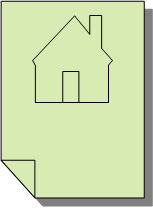
\includegraphics[width=0.25\textwidth]{figures/Homepage-icon.png}
% % 	\end{center}
% % 	\caption{Homepage icon}
% % 	\label{fig:homepageicon}
% % \end{figure}

% % \begin{table}[!ht]
% % 	\begin{center}
% % 		\caption{Configurations tested}
% % 		\label{tab:configstested}
% % 		\begin{tabular}{l|c} % <-- Alignments: 1st column left, 2nd middle and 3rd right, with vertical lines in between
% % 			\textbf{Configuration} & \textbf{Description}        \\
% % 			\hline
% % 			1                      & Simple test with one server \\
% % 			2                      & Simple test with one server \\
% % 		\end{tabular}
% % 	\end{center}
% % \end{table}
% % \todo[inline, backgroundcolor=kth-lightblue]{Konfigurationer testade}

% \section{Implementation …/Modeling/Simulation/…}
% \label{sec:implementationDetails}
% \todo[inline, backgroundcolor=kth-lightblue]{Implementering … / modellering / simulering / …}


% % \subsection{Some examples of coding}

% % Listing~\ref{lst:helloWorldInC} shows an example of a simple program written
% % in C code.

% % \begin{lstlisting}[language={C}, caption={Hello world in C code}, label=lst:helloWorldInC]
% % int main() {
% % printf("hello, world");
% % return 0;
% % }
% % 					 \end{lstlisting}


% % In contrast, Listing~\ref{lst:programmes} is an example of code in Python to
% % get a list of all of the programs at KTH.

% % \lstset{extendedchars=true}
% % \begin{lstlisting}[language={Python}, caption={Using a python program to
% %     access the KTH API to get all of the programs at KTH}, label=lst:programmes]
% % KOPPSbaseUrl = 'https://www.kth.se'

% % def v1_get_programmes():
% %     global Verbose_Flag
% %     #
% %     # Use the KOPPS API to get the data
% %     # note that this returns XML
% %     url = "{0}/api/kopps/v1/programme".format(KOPPSbaseUrl)
% %     if Verbose_Flag:
% %         print("url: " + url)
% %     #
% %     r = requests.get(url)
% %     if Verbose_Flag:
% %         print("result of getting v1 programme: {}".format(r.text))
% %     #
% %     if r.status_code == requests.codes.ok:
% %         return r.text           # simply return the XML
% %     #
% %     return None
% % 					 \end{lstlisting}


% \cleardoublepage
% \chapter{Results and Analysis}
% \label{ch:resultsAndAnalysis}
% \todo[inline, backgroundcolor=kth-lightblue]{svensk: Resultat och Analys}

% \todo[inline]{
% 	Sometimes this is split into two chapters.\\

% 	Keep in mind: How you are going to evaluate what you have done? What are your metrics?\\
% 	Analysis of your data and proposed solution\\
% 	Does this meet the goals which you had when you started?
% }

% In this chapter, we present the results and discuss them.

% \todo[inline, backgroundcolor=kth-lightblue]{I detta kapitel presenterar vi resultatet och diskutera dem.\\
% 	Ibland delas detta upp i två kapitel.\\
% 	Hur du ska utvärdera vad du har gjort? Vad är din statistik?\\
% 	Analys av data och föreslagen lösning\\
% 	Innebär detta att uppnå de mål som du hade när du började?
% }

% \section{Major results}
% \todo[inline, backgroundcolor=kth-lightblue]{Huvudsakliga resultat}

% Some statistics of the delay measurements are shown in Table~\ref{tab:delayMeasurements}.
% The delay has been computed from the time the GET request is received until the response is sent.

% \todo[inline, backgroundcolor=kth-lightblue]{Lite statistik av mätningarna fördröjnings visas i Tabell~\ref{tab:delayMeasurements}. Förseningen har beräknats från den tidpunkt då begäran GET tas emot fram till svaret skickas.}

% % \begin{table}[!ht]
% % 	\begin{center}
% % 		\caption{Delay measurement statistics}
% % 		\label{tab:delayMeasurements}
% % 		\begin{tabular}{l|S[table-format=4.2]|S[table-format=3.2]} % <-- Alignments: 1st column left, 2nd middle and 3rd right, with vertical lines in between
% % 			\textbf{Configuration} & \textbf{Average delay (ns)} & \textbf{Median delay (ns)} \\
% % 			\hline
% % 			1                      & 467.35                      & 450.10                     \\
% % 			2                      & 1687.5                      & 901.23                     \\
% % 		\end{tabular}
% % 	\end{center}
% % \end{table}
% % \todo[inline, backgroundcolor=kth-lightblue]{Fördröj mätstatistik}
% % \todo[inline, backgroundcolor=kth-lightblue]{Konfiguration | Genomsnittlig fördröjning (ns) | Median fördröjning (ns)}

% % Figure \ref{fig:processing_vs_payload_length} shows and example of the
% % performance as measured in the experiments.

% % \begin{figure}[!ht]
% % 	% GNUPLOT: LaTeX picture
% % 	\setlength{\unitlength}{0.240900pt}
% % 	\ifx\plotpoint\undefined\newsavebox{\plotpoint}\fi
% % 	\begin{picture}(1500,900)(0,0)
% % 		\sbox{\plotpoint}{\rule[-0.200pt]{0.400pt}{0.400pt}}%
% % 		\put(171.0,131.0){\rule[-0.200pt]{4.818pt}{0.400pt}}
% % 		\put(151,131){\makebox(0,0)[r]{ 1.5}}
% % 		\put(1419.0,131.0){\rule[-0.200pt]{4.818pt}{0.400pt}}
% % 		\put(171.0,212.0){\rule[-0.200pt]{4.818pt}{0.400pt}}
% % 		\put(151,212){\makebox(0,0)[r]{ 2}}
% % 		\put(1419.0,212.0){\rule[-0.200pt]{4.818pt}{0.400pt}}
% % 		\put(171.0,292.0){\rule[-0.200pt]{4.818pt}{0.400pt}}
% % 		\put(151,292){\makebox(0,0)[r]{ 2.5}}
% % 		\put(1419.0,292.0){\rule[-0.200pt]{4.818pt}{0.400pt}}
% % 		\put(171.0,373.0){\rule[-0.200pt]{4.818pt}{0.400pt}}
% % 		\put(151,373){\makebox(0,0)[r]{ 3}}
% % 		\put(1419.0,373.0){\rule[-0.200pt]{4.818pt}{0.400pt}}
% % 		\put(171.0,454.0){\rule[-0.200pt]{4.818pt}{0.400pt}}
% % 		\put(151,454){\makebox(0,0)[r]{ 3.5}}
% % 		\put(1419.0,454.0){\rule[-0.200pt]{4.818pt}{0.400pt}}
% % 		\put(171.0,534.0){\rule[-0.200pt]{4.818pt}{0.400pt}}
% % 		\put(151,534){\makebox(0,0)[r]{ 4}}
% % 		\put(1419.0,534.0){\rule[-0.200pt]{4.818pt}{0.400pt}}
% % 		\put(171.0,615.0){\rule[-0.200pt]{4.818pt}{0.400pt}}
% % 		\put(151,615){\makebox(0,0)[r]{ 4.5}}
% % 		\put(1419.0,615.0){\rule[-0.200pt]{4.818pt}{0.400pt}}
% % 		\put(171.0,695.0){\rule[-0.200pt]{4.818pt}{0.400pt}}
% % 		\put(151,695){\makebox(0,0)[r]{ 5}}
% % 		\put(1419.0,695.0){\rule[-0.200pt]{4.818pt}{0.400pt}}
% % 		\put(171.0,776.0){\rule[-0.200pt]{4.818pt}{0.400pt}}
% % 		\put(151,776){\makebox(0,0)[r]{ 5.5}}
% % 		\put(1419.0,776.0){\rule[-0.200pt]{4.818pt}{0.400pt}}
% % 		\put(171.0,131.0){\rule[-0.200pt]{0.400pt}{4.818pt}}
% % 		\put(171,90){\makebox(0,0){ 0}}
% % 		\put(171.0,756.0){\rule[-0.200pt]{0.400pt}{4.818pt}}
% % 		\put(298.0,131.0){\rule[-0.200pt]{0.400pt}{4.818pt}}
% % 		\put(298,90){\makebox(0,0){ 10}}
% % 		\put(298.0,756.0){\rule[-0.200pt]{0.400pt}{4.818pt}}
% % 		\put(425.0,131.0){\rule[-0.200pt]{0.400pt}{4.818pt}}
% % 		\put(425,90){\makebox(0,0){ 20}}
% % 		\put(425.0,756.0){\rule[-0.200pt]{0.400pt}{4.818pt}}
% % 		\put(551.0,131.0){\rule[-0.200pt]{0.400pt}{4.818pt}}
% % 		\put(551,90){\makebox(0,0){ 30}}
% % 		\put(551.0,756.0){\rule[-0.200pt]{0.400pt}{4.818pt}}
% % 		\put(678.0,131.0){\rule[-0.200pt]{0.400pt}{4.818pt}}
% % 		\put(678,90){\makebox(0,0){ 40}}
% % 		\put(678.0,756.0){\rule[-0.200pt]{0.400pt}{4.818pt}}
% % 		\put(805.0,131.0){\rule[-0.200pt]{0.400pt}{4.818pt}}
% % 		\put(805,90){\makebox(0,0){ 50}}
% % 		\put(805.0,756.0){\rule[-0.200pt]{0.400pt}{4.818pt}}
% % 		\put(932.0,131.0){\rule[-0.200pt]{0.400pt}{4.818pt}}
% % 		\put(932,90){\makebox(0,0){ 60}}
% % 		\put(932.0,756.0){\rule[-0.200pt]{0.400pt}{4.818pt}}
% % 		\put(1059.0,131.0){\rule[-0.200pt]{0.400pt}{4.818pt}}
% % 		\put(1059,90){\makebox(0,0){ 70}}
% % 		\put(1059.0,756.0){\rule[-0.200pt]{0.400pt}{4.818pt}}
% % 		\put(1185.0,131.0){\rule[-0.200pt]{0.400pt}{4.818pt}}
% % 		\put(1185,90){\makebox(0,0){ 80}}
% % 		\put(1185.0,756.0){\rule[-0.200pt]{0.400pt}{4.818pt}}
% % 		\put(1312.0,131.0){\rule[-0.200pt]{0.400pt}{4.818pt}}
% % 		\put(1312,90){\makebox(0,0){ 90}}
% % 		\put(1312.0,756.0){\rule[-0.200pt]{0.400pt}{4.818pt}}
% % 		\put(1439.0,131.0){\rule[-0.200pt]{0.400pt}{4.818pt}}
% % 		\put(1439,90){\makebox(0,0){ 100}}
% % 		\put(1439.0,756.0){\rule[-0.200pt]{0.400pt}{4.818pt}}
% % 		\put(171.0,131.0){\rule[-0.200pt]{0.400pt}{155.380pt}}
% % 		\put(171.0,131.0){\rule[-0.200pt]{305.461pt}{0.400pt}}
% % 		\put(1439.0,131.0){\rule[-0.200pt]{0.400pt}{155.380pt}}
% % 		\put(171.0,776.0){\rule[-0.200pt]{305.461pt}{0.400pt}}
% % 		\put(30,453){\rotatebox{-270}{\makebox(0,0){Processing time (ms)}}}
% % 		\put(805,29){\makebox(0,0){Payload size (bytes)}}
% % 		\put(868.0,131.0){\rule[-0.200pt]{0.400pt}{84.074pt}}
% % 		\put(995.0,131.0){\rule[-0.200pt]{0.400pt}{98.287pt}}
% % 		\put(1173.0,131.0){\rule[-0.200pt]{0.400pt}{118.041pt}}
% % 		\put(1325.0,131.0){\rule[-0.200pt]{0.400pt}{134.904pt}}
% % 		\put(1350.0,131.0){\rule[-0.200pt]{0.400pt}{137.795pt}}
% % 		\put(1439.0,131.0){\rule[-0.200pt]{0.400pt}{155.380pt}}
% % 	\end{picture}
% % 	\caption[A GNUplot figure]{Processing time vs. payload length}\vspace{0.5cm}
% % 	\label{fig:processing_vs_payload_length}
% % \end{figure}


% % Given these measurements, we can calculate our processing bit rate as the inverse of the time it takes to process an additional byte divided by 8 bits per byte:

% % \[
% % 	bitrate = \frac{1}{\frac{time_{byte}}{8}} = 20.03 \quad kb/s
% % \]

% \section{Reliability Analysis}
% \todo[inline, backgroundcolor=kth-lightblue]{Analys av reabilitet\\
% 	Reabilitet i metod och data}

% \section{Validity Analysis}
% \todo[inline, backgroundcolor=kth-lightblue]{Analys av validitet\\
% 	Validitet i metod och data}

% \cleardoublepage
% \chapter{Discussion}\todo[inline]{This can be a separate chapter or a section
% 	in the previous chapter.}
% \label{ch:discussion}
% \todo[inline, backgroundcolor=kth-lightblue]{Diskussion\\
% 	Förbättringsförslag?}

% \cleardoublepage
% \chapter{Conclusions and Future work}
% \label{ch:conclusionsAndFutureWork}
% \todo[inline, backgroundcolor=kth-lightblue]{Slutsats och framtida arbete}

% \todo[inline]{Add text to introduce the subsections of this chapter.}

% \section{Conclusions}
% \label{sec:conclusions}
% \todo[inline]{Describe the conclusions (reflect on the whole introduction given in Chapter 1).}
% \todo[inline, backgroundcolor=kth-lightblue]{Slutsatser}


% \todo[inline]{Discuss the positive effects and the drawbacks.\\
% 	Describe the evaluation of the results of the degree project.\\
% 	Did you meet your goals?\\
% 	What insights have you gained?\\
% 	What suggestions can you give to others working in this area?\\
% 	If you had it to do again, what would you have done differently?}

% \todo[inline, backgroundcolor=kth-lightblue]{Träffade du dina mål?\\
% 	Vilka insikter har du fått?\\
% 	Vilka förslag kan du ge till andra som arbetar inom detta område?
% 	Om du hade att göra igen, vad skulle du ha gjort annorlunda?}

% \section{Limitations}
% \label{sec:limitations}
% \todo[inline]{What did you find that limited your
% 	efforts? What are the limitations of your results?}
% \todo[inline, backgroundcolor=kth-lightblue]{Begränsande faktorer\\
% 	Vad gjorde du som begränsade dina ansträngningar? Vilka är begränsningarna i dina resultat?}

% \section{Future work}
% \label{sec:futureWork}
% \todo[inline]{Describe valid future work that you or someone else could or should do.\\
% 	Consider: What you have left undone? What are the next obvious things to be done? What hints can you give to the next person who is going to follow up on your work?
% }
% \todo[inline, backgroundcolor=kth-lightblue]{Vad du har kvar ogjort?\\
% 	Vad är nästa självklara saker som ska göras?\\
% 	Vad tips kan du ge till nästa person som kommer att följa upp på ditt arbete?
% }


% Due to the breadth of the problem, only some of the initial goals have been
% met. In these section we will focus on some of the remaining issues that
% should be addressed in future work. ...

% \subsection{What has been left undone?}
% \label{what-has-been-left-undone}

% The prototype does not address the third requirment, i.e., a yearly
% unavailability of less than 3 minutes, this remains an open problem. ...

% \subsubsection{Cost analysis}

% The current prototype works, but the performance from a cost perspective makes
% this an impractical solution. Future work must reduce the cost of this
% solution, to do so a cost analysis needs to first be done. ...

% \subsubsection{Security}

% A future research effort is needed to address the security holes that results
% from using a self-signed certificate. Page filling text mass. Page filling
% text mass. ...


% \subsection{Next obvious things to be done}

% In particular, the author of this thesis wishes to point out xxxxxx remains as
% a problem to be solved. Solving this problem is the next thing that should be
% done. ...

% \section{Reflections}
% \label{sec:reflections}
% \todo[inline]{What are the relevant economic, social,
% 	environmental, and ethical aspects of your work?
% }
% \todo[inline, backgroundcolor=kth-lightblue]{Reflektioner}
% \todo[inline, backgroundcolor=kth-lightblue]{Vilka är de relevanta ekonomiska, sociala, miljömässiga och etiska aspekter av ditt arbete?}


% One of the most important results is the reduction in the amount of
% energy required to process each packet while at the same time reducing the
% time required to process each packet.

% % The thesis contributes to the \gls{UN}\enspace\glspl{SDG} numbers 1 and 9 by
% xxxx.




% \noindent\rule{\textwidth}{0.4mm}
% \todo[inline]{In the references, let Zotero or other tool fill this
% 	in for you. I suggest an extended version of the IEEE  style, to include
% 	URLs, DOIs, ISBNs, etc., to make it easier for your reader to find
% 	them. This will make life easier for your opponents and examiner. \\

% 	IEEE Editorial Style Manual: \url{https://www.ieee.org/content/dam/ieee-org/ieee/web/org/conferences/style_references_manual.pdf}
% }
% \todo[inline, backgroundcolor=kth-lightblue]{Låt Zotero eller annat verktyg fylla i det h��r för dig. Jag föreslår en utökad version av IEEE stil - att inkludera webbadresser, DOI, ISBN etc. - för att göra det lättare för läsaren att hitta dem. Detta kommer att göra livet lättare för dina motståndare och examinator.}

% \cleardoublepage
% % Print the bibliography (and make it appear in the table of contents)
% \renewcommand{\bibname}{References}
% \addcontentsline{toc}{chapter}{References}

% \ifbiblatex
% 	%\typeout{Biblatex current language is \currentlang}
% 	\printbibliography[heading=bibintoc]
% \else
% 	\bibliography{references}
% \fi




% \cleardoublepage
% \appendix
% \renewcommand{\chaptermark}[1]{\markboth{Appendix \thechapter\relax:\thinspace\relax#1}{}}
% \chapter{Something Extra}
% \todo[inline, backgroundcolor=kth-lightblue]{svensk: Extra Material som Bilaga}

% \section{Just for testing KTH colors}
% \ifdigitaloutput
% 	\textbf{You have selected to optimize for digital output}
% \else
% 	\textbf{You have selected to optimize for print output}
% \fi
% \begin{itemize}[noitemsep]
% 	\item Primary color
% 	      \begin{itemize}
% 		      \item \textcolor{kth-blue}{kth-blue \ifdigitaloutput
% 				            actually Deep sea
% 			            \fi} {\color{kth-blue} \rule{0.3\linewidth}{1mm} }\\

% 		      \item \textcolor{kth-blue80}{kth-blue80} {\color{kth-blue80} \rule{0.3\linewidth}{1mm} }\\
% 	      \end{itemize}

% 	\item  Secondary colors
% 	      \begin{itemize}[noitemsep]
% 		      \item \textcolor{kth-lightblue}{kth-lightblue \ifdigitaloutput
% 				            actually Stratosphere
% 			            \fi} {\color{kth-lightblue} \rule{0.3\linewidth}{1mm} }\\

% 		      \item \textcolor{kth-lightred}{kth-lightred \ifdigitaloutput
% 				            actually Fluorescence\fi} {\color{kth-lightred} \rule{0.3\linewidth}{1mm} }\\

% 		      \item \textcolor{kth-lightred80}{kth-lightred80} {\color{kth-lightred80} \rule{0.3\linewidth}{1mm} }\\

% 		      \item \textcolor{kth-lightgreen}{kth-lightgreen \ifdigitaloutput
% 				            actually Front-lawn\fi} {\color{kth-lightgreen} \rule{0.3\linewidth}{1mm} }\\

% 		      \item \textcolor{kth-coolgray}{kth-coolgray \ifdigitaloutput
% 				            actually Office\fi} {\color{kth-coolgray} \rule{0.3\linewidth}{1mm} }\\

% 		      \item \textcolor{kth-coolgray80}{kth-coolgray80} {\color{kth-coolgray80} \rule{0.3\linewidth}{1mm} }
% 	      \end{itemize}
% \end{itemize}

% \textcolor{black}{black} {\color{black} \rule{\linewidth}{1mm} }

% %% The following label is necessary for computing the last page number of the body of the report to include in the "For DIVA" information
% \label{pg:lastPageofMainmatter}

% \clearpage
% \fancyhead{}  % Do not use header on this extra page or pages
\section*{For DIVA}
\lstset{numbers=none} %% remove any list line numbering
% \divainfo{pg:lastPageofPreface}{pg:lastPageofMainmatter}
\end{document}
